\documentclass[twoside,numberorder]{csbachelor}

%==============================================================
%==============================================================

\usepackage{url}
\usepackage{subfigure}


\usepackage[hidelinks]{hyperref}
\setlength{\LTpre}{1em}
\setlength{\LTpost}{1em}

\usepackage{tikz}
\usetikzlibrary{arrows,backgrounds,fit,shapes}
\tikzstyle{layer} = [draw, dashed]
\tikzstyle{block} = [draw, rectangle, minimum height=2em]
\tikzset{>=latex}

\usepackage{listings}
\usepackage{color}
\usepackage{float}


%New colors defined below
\definecolor{codegreen}{rgb}{0,0.6,0}
\definecolor{codegray}{rgb}{0.5,0.5,0.5}
\definecolor{codepurple}{rgb}{0.58,0,0.82}
\definecolor{backcolour}{rgb}{0.95,0.95,0.92}

%Code listing style named "mystyle"
\lstdefinestyle{mystyle}{
  backgroundcolor=\color{backcolour},   commentstyle=\color{codegreen},
  keywordstyle=\color{magenta},
  numberstyle=\tiny\color{codegray},
  stringstyle=\color{codepurple},
  basicstyle=\ttfamily\footnotesize,
  breakatwhitespace=false,         
  breaklines=true,                 
  captionpos=b,                    
  keepspaces=true,                 
  numbers=left,                    
  numbersep=5pt,                  
  showspaces=false,                
  showstringspaces=false,
  showtabs=false,                  
  tabsize=2
}
%"mystyle" code listing set
\lstset{style=mystyle}


% 一些全局工具的定义
\DeclareMathOperator*{\argmin}{arg\,min}
\DeclareMathOperator*{\argmax}{arg\,max}

%==============================================================
%==============================================================

\begin{document}

%==============================================================
%==============================================================
  \sduttitle{在线考试系统}{Online Examination System}
  \sdutdate{2021年6月}{June,2021}
  \sdutschool{计算机科学与技术学院}{Computer Science And Technology}
  \sdutmajor{计算机科学与技术}{Computer Science And Technology}
  \sdutstudentname{韩勇}{Yong Han}
  \sdutstudentid{17110543012}{17110543012}
  \instructor{曹雁锋}{Yanfeng Cao}


%==============================================================

  {
    \pagestyle{empty}

    {
  \setlength{\parindent}{0em}

  {
    \linespread{1}
    \begin{flushleft}
      
\includegraphics[height=23.8mm]{data/cover-zh/logo.eps}
    \end{flushleft}

    \vspace{2em}
    
    {
      \heiti\sishiwu\bfseries
      \centering
      毕~~业~~论~~文 \par
    }
    \vspace{6em}
    
    {
      \heiti\erhao\bfseries
      \centering
      {\sduttitlec} \par
    }
    
  }
  

  \vspace{12em}

  {
    \linespread{1.6}
    \songti\xiaosan\bfseries
    \centering
    \newlength{\titlelength}
    \setlength{\titlelength}{18em}
    学 \qquad 院: \; \underline{\makebox[\titlelength]{\sdutschoolc}}\\
    专 \qquad 业: \; \underline{\makebox[\titlelength]{\sdutmajorc}} \\
    学生姓名: \; \underline{\makebox[\titlelength]{\sdutstudentnamec}} \\
    学 \qquad 号: \; \underline{\makebox[\titlelength]{\sdutstudentidc}} \\
    指导老师: \; \underline{\makebox[\titlelength]{\instructorc}} \par
  }
  \vfill
  {
    \songti\sihao\bfseries
      \centering
      \sdutdatec \par
  }
}

    \cleardoublepage
    {
  \setlength{\parindent}{0em}

  {
    \linespread{1}
    \begin{flushleft}
      
\includegraphics[height=23.8mm]{data/cover-zh/logo.eps}
    \end{flushleft}

    \vspace{2em}
    
    {
      \heiti\sishiwu\bfseries
      \centering
      Graduation~~Thesis \par
    }
    \vspace{6em}
    
    {
      \heiti\erhao\bfseries
      \centering
      {\sduttitlee} \par
    }
    
  }

 

  \vspace{12em}

  {
    \linespread{1.6}
    \begin{center}
    \xiaosan
    \newlength{\majorlength}
    \setlength{\majorlength}{16em}
    \begin{tabular}{l l}
    College : \underline{\makebox[\majorlength]{\sdutschoole}} \\
    Major : \underline{\makebox[\majorlength]{\sdutmajore}} \\
    Author : \underline{\makebox[\majorlength]{\sdutstudentnamee}} \\
    Student ID : \underline{\makebox[\majorlength]{\sdutstudentide}} \\
    Instructor : \underline{\makebox[\majorlength]{\instructore}} \\
    \end{tabular} \par
    \end{center}
  }
  \vfill
  {
    \songti\sihao\bfseries
      \centering
      \sdutdatee \par
  }
}


    \cleardoublepage

    \include{data/agreement}
    \cleardoublepage
  }
  
  {
    \frontmatter

    \pagestyle{frontmatter}
    \makeatletter
      \let\ps@plain\ps@frontmatter
    \makeatother

    \chapter{摘要}

随着计算机技术的发展,计算机和网络技术越来越广泛的应用于各个领域,改变着人们的学习、工作和生活。如今大学的规模不断扩大,
学生不断增加,但学校仍采用传统的笔试模式组织考试,笔试存在很多问题,例如复杂考试程序和容易出现的错误。
\par
随着计算机时代的飞速发展应用,网络技术变得更加成熟并提高了考试质量,方便学生参加考试,并感到公义,公证和开放性。
目前许多考试已经采用无纸化考试方式,如计算机等级考试、微软的MCSE、Cisco的CCNA等。因此,开发在线考试系统很有必要。
根据在线考试系统的操作重点,本文将介绍功能要求,使用图表通过以下方式表达和描述案例图。在系统设计中,本文将详细设计功能模块通过使用类图,以及数据库采用的设计实体类图,ER图和数据库表结构体。


    \tableofcontents

    \newpage
    \thispagestyle{empty}
  }

  {
    \mainmatter

    \pagestyle{mainmatter}
    \makeatletter
      \let\ps@plain\ps@mainmatter
    \makeatother

    \chapter{引言}

\section{课题的来源及意义}
在互联网飞速发展的今天,计算机和网络技术越来越广泛的应用于各个领域,改变着人们的学习、工作和生活。
随着教育现代化步伐的加快和计算机辅助教学的广泛应用,利用计算机的强大功能参与教学已成为教育工作者和教育科研人员广泛关注的研究领域。
目前,社会各个行业需要人才,而人才选拔的重要途径就是通过考试来判定。
现阶段,学校的考试大都是采用传统的考试方式:由老师出题,经复印后,学生纸上答题,老师人工阅卷,以及学生的学习状态分析也是人工进行的。
通常的出卷方式是参与教学的教师根据自己的知识、经验、风格来收集、选取并编制试题,这样做虽然试题的效率、信用度高,但同样存在着一定的缺点,主要表现在由于人为因素的不确定性,
可能会造成选题范围过于狭窄;耗费教师大量的时间、精力;不利于实现考、教分离。传统的考试方式由于工作量大从而容易出错。不仅如此,这样的考试方式不仅给老师带来了繁重的任务,
而且使得老师的工作效率大打折扣,不利于老师工作效率的提高。与传统的考试模式相比,在线考试具有无可比拟的优越性,具体优点如下:
\begin{enumerate}
	\item 将教师从繁重的出卷、阅卷、评卷的繁重工作中解脱出来,教师的工作效率大幅提高,减少人为主观意志对评分的影响,有效提高教育质量。
	\item 学生在平时的学习中,及时的在网上进行自我测试,在学习上能够查缺补漏,激发学生的学习兴趣,为学生的学习带来更多的方便。
	\item 系统实现自动组卷、客观题自动评分,使考试真正做到客观、公平、公正,真正实现考、教分离。
\end{enumerate}
\section{国内外的发展情况}
计算机考试系统的实现,将教师从繁琐的出题、监考、阅卷、试卷分析和成绩统计的传统考试中解脱出来,充分体现了准确、客观、公正、快速、简捷等特点。
20世纪70年代,美国考试委员会着手进行计算机模拟考试的研究工作,并于1983年编制出有效的模拟考试系统,当时的名称是计算机辅助考试系统。
1990年8月,美国加利福尼亚、得克萨斯等十个州创建各州以及各高等院校相互认可的学位证书以及相应的教学体系,从而正式拉开网络远程考试的序幕。
著名的考试机构有美国思而文学习系统有限公司。它是一家从事教育和计算机化考试服务的专业公司,在世界的6大洲140多个国家和地区有2200多个考试中心,
可用25种语言提供近百个不同类型,一千多种考试,每年全球参加计算机化考试的人数约400万。当今大部分的授证机构均委托思而文公司为其进行测试、评估。
最出名的网络教育案例,当属美国政府举办的TOFEL考试,目前在全球范围内,均可以通过国际互联网进行TOFEL培训与考试,大大减少了美国政府对于此项考试的开支,
并能更快速、准确地为期望进入美国学习的学生服务。目前美国约有 80 所大学允 许学生通过网络考试获得学位,另外,加拿大、英国等其它西方国家也在大力开展网络考试系统。
\par
与西方发达国家的突飞猛进相比,国内的计算机考试技术研究工作开展的相对较晚,但国内在网络远程教学研究工作发展相当迅速。
目前各高等院校如清华大学、北京 大学、上海复旦大学、同济大学、西安交通大学、华南理工大学、北京医科大学和湖南 大学等高校己陆续在网上设立了自己的考试系统,
并开展相关研究。国家信息产业部也开发了办公自动化证书CEAC远程考试系统、红旗 Linux 远程考试系统。通过对国内外计算机考试系统的考察和试用,我们发现它们具备以下特点:
\begin{itemize}
	\item C/S 结构和 B/S 结构并存,但基本都可以在网络上使用。
	\item 大都提供自动组卷和自动评卷功能,但水平参差不齐
	\item 考核软件使用仿真模拟环境和调用真实环境两者都有
	\item 均采 用了开放式试题库 , 扩充比较容易
	\item 对题库的分析管理部分都比较重 , 都提供了最基 本的功能
\end{itemize}
\section{课题开发的目标和内容}
\subsection{目标}
本课题设计是一个较为完善的在线的考试系统,并且拥有基本的用户管理。
\subsection{内容}
\begin{enumerate}
	\item 便捷建题:全面题型支持,客观题、主观题、自定义题型(A型题、阅读理解题、名词解释等);试题格式多样化,支持数学公式、化学分子式、图形图像、上下标、特殊符号全学科试题,完美解决数学公式、化学公式输出不失真;
	\item 题库管理:支持单人建设和多人共建一门题库,完善的辅助功能,严密的权限管理;
	\item 练习测试:学生课后练习或自学练习,老师可向学生开通一定比例的试题或手动挑选部分试题供学生练习,提供错题集和练习记录,理解和巩固相关知识点。提高学生练习的积极性,从而达到以练促学,以学促考的再次“翻转”;
	\item 组卷和排考:管理者基于试题库,支持组织试卷并通过安排考场、安排学生等简单流程即可完一场在线考试;
	\item 试卷评阅:客观题自动评阅,主观题由阅卷教师在线评阅,可根据题型逐题评阅,评阅时可分别针对试题给出评语;
	\item 教学分析:对学生成绩进行分析,形成评测报告;
	\item 监考功能:考生进入考试后,在考试过程中系统随机、自动抓拍五次考试照片,自动上传监控台存档;
\end{enumerate}





    \chapter{需求分析及可行性分析}

\section{需求分析}
考试是检测个人能力的一个重要手段,而常见的考试方式除了传统的纸笔考试外,还有随着互联网一起快速发展的在线考试。
传统考试有自己的独特优点,而在线考试也不遑多让,在考试系统中很快就抢占了不少的份额。
在线考试系统自从桌面系统被普及后就已经在被使用,从原来的局域网考试,到互联网考试,再到现在的手机在线考试,
无论是C/S考试软件架构,还是B/S Web考试软件架构,在线考试系统一直都在不断发展,并在最近几年被广泛应用。
\par
在线考试快速发展的一个主要原因就是使用方便,考试成本低,节约时间。
同时在线考试系统能够对考生答卷中绝大多数题目智能阅卷并评分,大大减少了人力工作,正好适合学校平时练习和有考核需求的社会机构使用。
此外,在COVID-19大流行中,教育是唯一获得可观市场收入的行业。由于北美不同国家/地区的全国封锁,各种学校和大学都在远程进行考试。所有私立和公共教育机构均被迫中止课堂学习并适应在线学习。
\section{可行性分析}
经济可行性:随着经济技术的快速发展,目前硬件价格普遍下跌,宽带网大力建设,所以只需要在软件开发上面投入少许经费就可以了。
系统能降低管理费用和劳动费用,提高人员利用率,保证工作质量,人力资源合理分配,达到资源优化。这不仅给教师工作带来方便,
同时也满足了不同客户的不同需求,提高了数据的安全性、共享性,降低了预算,提高了工作效率,因此经济上可行。
\par
技术可行性:虽然本人在前后端开发经验上有所不足,但具有较强的动手能力,能够对老师所教导的内容进行融会贯通。
本次最大的挑战即时在系统中加入遗传算法并且平衡各方面相互制约的影响因素,使系统更加完善,我相信在老师的教导下能够快速且高质量的完成本次课题。
\par
管理可行性:目前,在线测试系统正在被更多的人所认可。在线测试系统能够实现无纸化考试,可以满足任何授权的考生随时随地考试并迅速获得成绩,
同时也大大减轻了教师出题和判卷等繁重的工作量。而且所面向的群体不止局限于学生,面向对象更广,为成年人创造了有利条件。



    \chapter{系统主要功能设计与实现}

\section{开发及运行环境}
\begin{enumerate}
	\item[(1)] 项目开发环境:
		\begin{itemize}
			\item CPU 最低Intel Core i5 4590或同等性能芯片。
			\item 推荐 Intel Core i7 7700或AMD同等性能芯片及以上。
			\item 内存 最低8GB(推荐16GB及以上)。
			\item 硬盘 需要10GB以上的可用空间(固态硬盘为宜)。
			\item 网络 接入互联网下行20Mbps及以上,上行10Mbps及以上。
			\item 操作系统 macOS Big Sur Version 11.3.1。
			\item 基本软件 JDK-11、MariaDB、Redis、ElasticSearch和Maven。
		\end{itemize}
	\item[(2)] 软件部署环境:
		\begin{itemize}
			\item CPU 最低Intel Core i5 4590或同等性能芯片。
			\item 推荐 Intel Core i7 7700 或AMD同等性能芯片及以上。
			\item 内存 最低8GB(推荐16GB及以上。
			\item 硬盘 需要10GB以上的可用空间(固态硬盘为宜)。
			\item 网络 接入互联网下行20Mbps及以上,上行10Mbps及以上。
		\end{itemize}
\end{enumerate}

\section{系统架构设计}
系统采用B/S(Browser/Server,浏览器/服务器)方式的网络结构,统一采用如Chrome一类的浏览器,通过访问前端服务器获取页面,
前端服务器通过Json向业务服务器发送请求,由Nginx负载均衡分发给各个业务服务器,业务服务器对请求处理后,将结果返回给客户端。
架构设计如图\ref{figure:jiagou}所示。
\begin{figure}[!htbp]
\centering
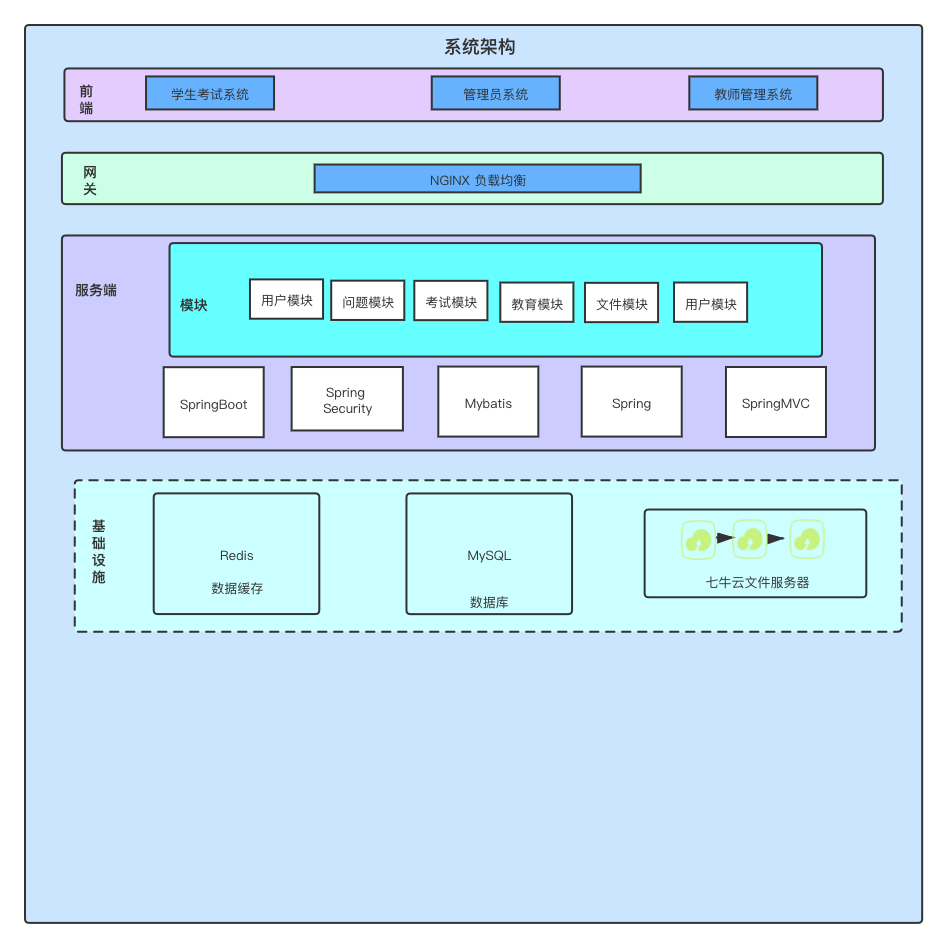
\includegraphics[width=0.6\textwidth,keepaspectratio]{data/chapter-2/jiagou.png}
\caption{系统架构}
\label{figure:jiagou}
\end{figure}

\section{系统各个功能模块的分析与设计}

\subsection{}
    \chapter{数据库设计}
采用 MariaDB 作为系统数据库存储所有系统有关的数据。数据库表和数据库表中的字段的命名规则如下。
\begin{enumerate}
	\item[(1)] 数据库表由符合相应模块功能含义的英文单词组成。
	\item[(2)] 字段命名由相应的表名称的缩写和符合字段含义的英文或拼音组成。
	\item[(3)] 命名应遵循“见名知意”的原则
\end{enumerate}
\section{数据库需求分析}
用户的需求具体体现在各种信息的提供、保存、更新和查询,这就哟啊求数据哭结构能充分满足各种信息的输入输出,收集基本数据、数据结构以及数据处理的流程。针对在线考试系统的核心流程,
通过对用户操作流程的分析,主要可以有以下所示的数据项和数据结构。
\begin{enumerate}
	\item[(1)] 用户信息。ID、昵称、密码、真实姓名、年龄、性别、生日、手机号、角色等。
	\item[(2)] 试卷表。ID、试卷名、试卷类型、试卷总分、试卷开始时间、结束时间、试题总数、建议时间、创建人、创建时间等。
	\item[(3)] 试题表。ID、试题类型、班级、分数、难度、正确答案、描述等。
	\item[(4)] 班级表。班级ID、班级名称。
	\item[(5)] 考试表。考试名、考试班级、考试描述、考试创建人、考试创建时间。
	\item[(6)] 答题表。试卷ID、试卷名字、试卷类型、答题人、得分、满分、详细描述。 
\end{enumerate}
\section{数据库概念结构设计}
根据数据库需求分析中的数据项和数据结构,设计了满足系统各个需求的实体,以及它们之间的关系.根据需求分析规划出的实体有用户实体、班级实体、试卷实体、题目实体、试题答案试题、用户回答实体。
\par
实体之间关系的E-R如图\ref{figure:er}所示
\begin{figure}[!htbp]
\centering
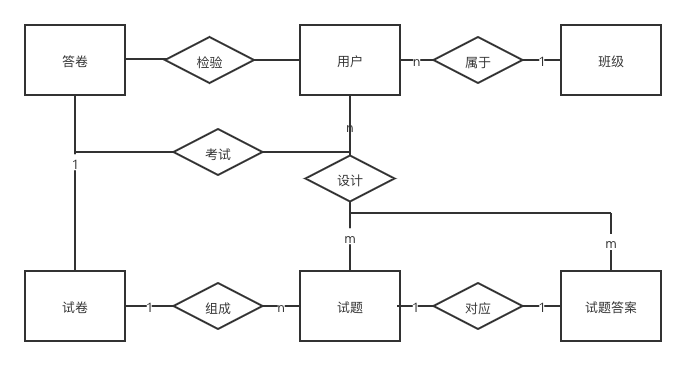
\includegraphics[width=0.6\textwidth,keepaspectratio]{data/chapter-4/er2.png}
\caption{E-R图}
\label{figure:er}
\end{figure}\section{数据库物理结构设计}
数据库物理设计阶段的任务是根据具体计算机系统和硬件等的特点,为给定的数据库模型确定合理的存储结构和存取方法。
\par
根据逻辑结构设计确定数据库中各个表及字段类型如下
\begin{enumerate}
	\item[(1)] User表,用户表用于存储用户的基本信息。如图表\ref{table:user}所示。
	\begin{table}[!htbp]
		\centering
		\begin{tabular}{|c|c|c|c|}
			\hline
			字段名 & 类型(长度) & 是否可以为空 & 说明 \\
			\hline
			ID & int(11) & PRIMARY KEY & 唯一标识 \\
			\hline
			user\_name & varchar(255) & YES & 用户名 \\
			\hline
			password & varchar(255) & YES & 密码 \\
			\hline
			real\_name & varchar(255) & YES & 真实姓名 \\
			\hline
			age & int(11) & YES	 & 年龄 \\
			\hline
			sex & int(11) & YES & 性别 \\
			\hline
			birth\_day & datetime & YES & 生日 \\
			\hline
			phone & varchar(255) & YES & 手机号 \\
			\hline
			role & int(11) & YES & 角色 \\
			\hline
			status & int(11) & YES & 状态 \\
			\hline
			image\_path & varchar(255) & YES & 头像 \\
			\hline
			create\_time & datetime & YES & 创建时间 \\
			\hline
			modify\_time & datetime & YES & 最后一次修改时间 \\
			\hline
			last\_active\_time & datetime & YES & 最后一次活动时间 \\
			\hline
			deleted & tinyint(1) & YES & 是否删除 \\
			\hline
			enabled & tinyint(1) & YES & 是否启用 \\
			\hline
			locked & tinyint(1) & YES & 是否锁定 \\
			\hline
		\end{tabular}
		\caption{用户表}
		\label{table:user}
	\end{table}
	\item[(2)] 班级表,班级表用于存储班级的基本信息。如图表\ref{table:class}所示。
	\begin{table}[!htbp]
		\centering
		\begin{tabular}{|c|c|c|c|}
			\hline
			字段名 & 类型(长度) & 是否可以为空 & 说明 \\
			\hline
			ID & int(11) & PRIMARY KEY & 唯一标识 \\
			\hline
			name & varchar(255) & YES & 班级名 \\
			\hline
			deleted & tinyint(1) & YES & 是否删除 \\
			\hline
		\end{tabular}
		\caption{班级表}
		\label{table:class}
	\end{table}
	\item[(3)] 试题表,试题表主要用于存储实体的基本信息,主要有ID、试题类型、班级、分数、难度、正确答案、描述等。如图表\ref{table:question}所示。
	\begin{table}[!htbp]
		\centering
		\begin{tabular}{|c|c|c|c|}
			\hline
			字段名 & 类型(长度) & 是否可以为空 & 说明 \\
			\hline
			ID & int(11) & PRIMARY KEY & 唯一标识 \\
			\hline
			score & int(11) & YES & 分数 \\
			\hline
			grade\_level & int(11) & YES & 班级 \\
			\hline
			difficult & int(11) & YES & 难度 \\
			\hline
			correct & text & YES & 正确答案 \\
			\hline
			info\_text\_content\_id & int(11) & YES & 上下文唯一标识符 \\
			\hline
			create\_user & int(11) & YES & 创建人 \\
			\hline
			status & int(11) & YES & 状态 \\
			\hline
			create\_time & datetime & YES & 创建时间 \\
			\hline
			deleted & tinyint(1) & YES & 是否删除 \\
			\hline
		\end{tabular}
		\caption{题目表}
		\label{table:question}
	\end{table}
	\item[(4)] 试卷表,试卷表主要用于存储试卷实体的基本信息。试卷ID、试卷名称和内容。如图表\ref{table:paper}所示。
	\begin{table}[!htbp]
		\centering
		\begin{tabular}{|c|c|c|c|}
			\hline
			字段名 & 类型(长度) & 是否可以为空 & 说明 \\
			\hline
			ID & int(11) & PRIMARY KEY & 唯一标识 \\
			\hline
			name & varchar(255) & YES & 名字 \\
			\hline
			paper\_type & int(11) & YES & 试卷类型 \\
			\hline
			grade\_level & int(11) & YES & 班级 \\
			\hline
			score & int(11) & YES & 分数 \\
			\hline
			question\_count & int(11) & YES & 问题数 \\
			\hline
			suggest\_time & int(11) & YES & 建议时间 \\
			\hline
			limit\_start\_time & datetime & YES & 开始时间 \\
			\hline
			limit\_end\_time & datetime & YES & 结束时间 \\
			\hline
			frame\_text\_content\_id & int(11) & YES & 内容ID \\
			\hline
			create\_user & int(11) & YES & 创建人 \\
			\hline
			create\_time & datetime & YES & 创建时间 \\
			\hline
			deleted & bit(1) & YES & 是否删除 \\
			\hline
			task\_exam\_id & int(11) & YES & 考试ID \\
			\hline
		\end{tabular}
		\caption{试卷表}
		\label{table:paper}
	\end{table}
	\item[(5)] 考试表,考试表用于存储考试的基本信心。主要包括考试名、考试班级、考试描述、考试创建人、考试创建时间。如图表\ref{table:exam}所示。
	\begin{table}[!htbp]
		\centering
		\begin{tabular}{|c|c|c|c|}
			\hline
			字段名 & 类型(长度) & 是否可以为空 & 说明 \\
			\hline
			ID & int(11) & PRIMARY KEY & 唯一标识 \\
			\hline
			title & varchar(255) & YES & 标题 \\
			\hline
			grade\_level & int(11) & YES & 班级 \\
			\hline
			frame\_text\_content\_id & int(11) & YES & 内容ID \\
			\hline
			create\_user & int(11) & YES & 创建人 \\
			\hline
			create\_time & datetime & YES & 创建时间 \\
			\hline
			deleted & bit(1) & YES & 是否删除 \\
			\hline
			create\_user\_name & varchar(255) & YES & 创建人姓名 \\
			\hline
		\end{tabular}
		\caption{考试表}
		\label{table:exam}
	\end{table}
	\item[(6)] 答题表,答题表用于存储答题的基本信息。主要包括试卷ID、试卷名字、试卷类型、答题人、得分、满分、详细描述。 如图表\ref{table:dati}所示。
	\begin{table}[!htbp]
		\centering
		\begin{tabular}{|c|c|c|c|}
			\hline
			字段名 & 类型(长度) & 是否可以为空 & 说明 \\
			\hline
			ID & int(11) & PRIMARY KEY & 唯一标识 \\
			\hline
			question\_id & int(11) & YES & 问题的唯一标识 \\
			\hline
			exam\_paper\_id & int(11) & YES & 试卷的唯一标识 \\
			\hline
			exam\_paper\_answer\_id & int(11) & YES & 试卷答案的唯一标识 \\
			\hline
			question\_type & int(11) & YES & 问题类型 \\
			\hline
			customer\_score & int(11) & YES & 用户分数 \\
			\hline
			question\_score & int(11) & YES & 问题分数 \\
			\hline
			question\_text\_content\_id & int(11) & YES & 问题内容ID \\
			\hline
			answer & varchar(255) & YES	 & 答案 \\
			\hline
			text\_content\_id & int(11) & YES & 描述ID \\
			\hline
			do\_right & bit(1) & YES & 是否正确 \\
			\hline
			create\_user & int(11) & YES & 创建人 \\
			\hline
			create\_time & datetime & YES & 创建时间 \\
			\hline
		\end{tabular}
		\caption{考试表}
		\label{table:dati}
	\end{table}
\end{enumerate}

    \chapter{系统实现}

\section{系统实现采用的主要技术方法}
\subsection{开发工具的选择}
编程环境选择IntelliJ IDEA。IntelliJ IDEA是Java编程语言开发的集成环境。
IntelliJ在业界被公认为最好的java开发工具,尤其在智能代码助手、代码自动提示、重构、JavaEE支持、各类版本工具(git、svn等)、
JUnit、CVS整合、代码分析、 创新的GUI设计等方面的功能可以说是超常的。IDEA是JetBrains公司的产品,这家公司总部位于捷克共和国的首都布拉格,
开发人员以严谨著称的东欧程序员为主。
\par
数据库软件选择MariaDB。MariaDB数据库管理系统是MySQL的一个分支,主要由开源社区在维护,采用GPL授权许可 MariaDB的目的是完全兼容MySQL,
包括API和命令行,使之能轻松成为MySQL的代替品。在存储引擎方面,使用XtraDB(英语:XtraDB)来代替MySQL的InnoDB。 
MariaDB由MySQL的创始人Michael Widenius(英语:Michael Widenius)主导开发,他早前曾以10亿美元的价格,将自己创建的公司MySQL AB卖给了SUN,
此后,随着SUN被甲骨文收购,MySQL的所有权也落入Oracle的手中。MariaDB名称来自Michael Widenius的女儿Maria的名字。
MariaDB基于事务的Maria存储引擎,替换了MySQL的MyISAM存储引擎,它使用了Percona的 XtraDB,InnoDB的变体,
分支的开发者希望提供访问即将到来的MySQL 5.4 InnoDB性能。这个版本还包括了 PrimeBase XT (PBXT) 和 FederatedX存储引擎。
\subsection{Spring 框架的特点}
Spring框架是一个开放源代码的J2EE应用程序框架,由Rod Johnson发起,是针对bean的生命周期进行管理的轻量级容器(lightweight container)。
Spring解决了开发者在J2EE开发中遇到的许多常见的问题,提供了功能强大IOC、AOP及Web MVC等功能。
Spring可以单独应用于构筑应用程序,也可以和Struts、Webwork、Tapestry等众多Web框架组合使用,并且可以与 Swing等桌面应用程序AP组合。
因此, Spring不仅仅能应用于J2EE应用程序之中,也可以应用于桌面应用程序以及小应用程序之中。Spring框架主要由七部分组成,
分别是 Spring Core、 Spring AOP、 Spring ORM、 Spring DAO、Spring Context、 Spring Web和 Spring Web MVC。
Spring主要有以下优点:
\par
\begin{enumerate}
	\item 非侵入式编程 \\
	Spring框架的API不会再业务逻辑上出现,即业务逻辑是POJO(Plain Ordinary Java Object)。由于业务逻辑中没有Spring的API,所以业务逻辑可以从Spring框架快速的移植到其他框架。
	\item 容器 \\
	Spring作为一个容器,可以管理对象的生命周期、对象与对象之间的依赖关系。可以通过配置文件来定义对象,以及设置其他对象的依赖关系。
	\item IoC \\
	控制反转(Inversion of Control),即创建被调用的实例不是由调用者完成,而是由Spring容器完成,并注入调用者。
当应用IoC,一个对象依赖的其他对象会通过被动的方式传递进来,而不是这个对象自己创建或查找依赖对象,即,不是对象从容器中查找依赖,而是容器在对象初始化时不等对象请求就主动将依赖传递给它。
	\item AOP \\
	面向切面编程,是一种编程思想,是面向对象编程OOP的补充。Spring提供面向对象编程的支持,允许通过分离应用的业务逻辑与系统级服务(日志和事务管理)进行开发。应用对象只实现他们应该做的(完成业务逻辑),并不负责其它的系统级关注点(日志或者事务的支持)。
可以把日志、安全、事务管理等服务理解成一个“切面”,把很多被业务逻辑反复使用的服务完全剥离出来,以达到复用。然后将“切面”动态的“织入”到业务逻辑中,让其享受此“切面”的服务。
\end{enumerate}
\section{开发环境的搭建}
\subsection{MariaDB数据库的优势}
MariaDB是MySQL的分支版本。它主要是由于MySQL在被Oracle公司收购时出现的问题而开发的。MariaDB是一个通用的数据库管理系统(DBMS),它具有可扩展的架构,可通过可插拔存储引擎支持大量的用例。它使用不同的存储引擎来支持不同的用例。
\par
MariaDB是一款开源的多线程关系数据库管理系统,在GNU公共许可证(GPL)下发布。其首席开发人员是Michael Monty Widenius,他也是MySQL AB的创始人之一。作为数据库系统,许多功能有助于MariaDB的普及。其速度是其最显着的特点之一。MariaDB也具有很强的可扩展性,能够处理数万张表和数十亿行数据。它还可以快速平稳地管理少量数据,方便小型企业或个人项目。另一个与前任不同的特点是专注于安全。MariaDB的内置功能包括操作和格式化文本,业务和统计计算,记录时间顺序信息,
\par
MariaDB服务器是世界上最流行的开源数据库之一。它在Debian和Ubuntu中可用,现在是Arch Linux,Manjaro,openSUSE,Red Hat Enterprise Linux,CentOS,Fedora和SUSE Linux Enterprise的默认数据库。作为世界上最广泛采用和广泛部署的产品之一,MariaDB服务器收到阿里巴巴,Facebook和谷歌等公司的捐款。最近,微软还联手支持MariaDB社区。以下是MariaDB的主要优势:
\begin{enumerate}
	\item MariaDB可用于GPL,LGPL和BSD。
	\item 它包括广泛的存储引擎选择,包括高性能存储引擎,用于与其他关系数据库管理系统(RDBMS)数据源一起工作。
	\item 它使用标准和流行的查询语言。
	\item MariaDB在许多操作系统上运行,并支持各种编程语言。
	\item 它提供对PHP的支持,PHP是最流行的Web开发语言之一。
	\item 它提供Galera群集技术。
	\item MariaDB还提供了很多在MySQL中不可用的操作和命令,并消除/取代了对性能产生负面影响的功能。
	\item 其他功能还包括多源复制,融合IO优化,表发现和联机更改表。
\end{enumerate}
\subsection{SpringBoot配置}
在开发本考试系统时,我将所有的运行时需要的配置都放在application.yml文件(即应用程序的配置文件)中。其核心代码如下:
\begin{lstlisting}
system:
  security-ignore-urls:
    - /api/admin/upload/configAndUpload
    - /api/admin/upload/auth
    - /api/student/user/register
  pwdKey:
    publicKey: 
    privateKey: 
  qn:
    url: http://image.hanblog.fun
    bucket: han-exam
    access-key: 
    secret-key: 

# datasource
spring:
  datasource:
    url: jdbc:mysql://localhost:3306/exam?useSSL=false&useUnicode=true&serverTimezone=Asia/Shanghai&characterEncoding=utf8&zeroDateTimeBehavior=convertToNull&allowPublicKeyRetrieval=true&allowMultiQueries=true
    username: root
    password: 123456
    driver-class-name: com.mysql.cj.jdbc.Driver

# mybatis
mybatis:
  mapper-locations: classpath:/mapping/*.xml
  configuration:
    log-impl: org.apache.ibatis.logging.stdout.StdOutImpl

#mybatis page helper
pagehelper:
  autoDialect: true
  closeConn: true
  reasonable: true
\end{lstlisting}
\section{主要功能模块}
系统由学生子系统、教师子系统和管理员子系统三部分组成。学生、教师、管理员三种不同的角色可以登录到对应的子系统。学生子系统包括在线考试/练习、成绩查询
考生信息管理、错题本等模块。教师子系统包括考试管理、试题管理、组卷管理、成绩管理、学生管理。管理员子系统包括考试管理、试题管理、组卷管理、成绩管理、用户管理。
下面将对登录模块、考试模块、考试管理模块、试题管理模块、组卷管理模块、成绩管理模块、个人信息管理模块进行分析阐述。
\subsection{登录模块}
该模块主要用于用户的身份认证。该模块是本系统非常重要的一部分,它接收用户提交的登录信息,并在用户信息表中检验是否有存在对应的用户和对应的权限。成功后向用户发放短时间内有效的Token令牌,
并将令牌存储到Redis缓存中。当用户再次发送请求是直接从缓存中判断用户身份以及权限。如图\ref{figure:login}所示。
\begin{figure}[H]
\centering
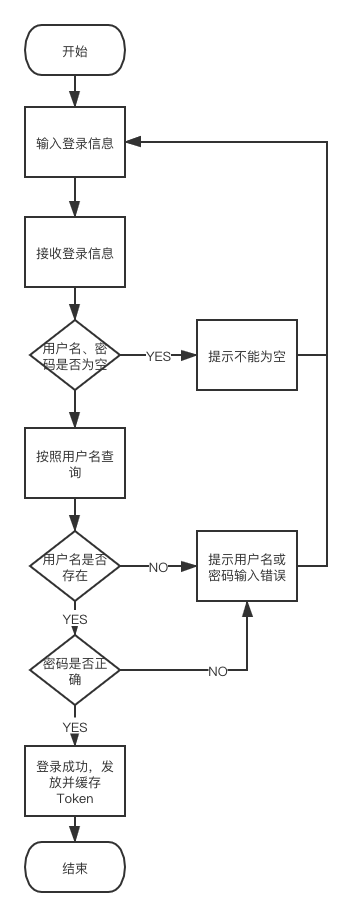
\includegraphics[width=0.4\textwidth,keepaspectratio]{data/chapter-5/login.png}
\caption{登录模块流程图}
\label{figure:login}
\end{figure}
\subsection{学生考试/练习模块}
该模块中列出了学生可以参加的所有练习和考试。学生选择其中一个考试/练习之后,系统开始计时,在考试过程中随机拍照并上传图片服务器,倒计时结束后自动交卷,
考生也可以在考试时间结束之前自行交卷。学生考试/练习模块流程图如\ref{figure:exam}所示。
\begin{figure}[H]
\centering
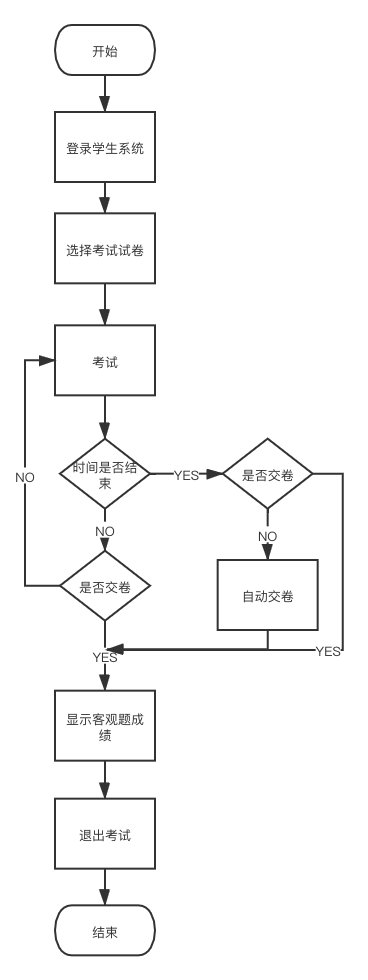
\includegraphics[width=0.5\textwidth,keepaspectratio]{data/chapter-5/exam.png}
\caption{考试模块流程图}
\label{figure:exam}
\end{figure}
\subsection{考试管理模块}
该模块主要用于添加、修改、删除考试信息。该模块结构图如图\ref{figure:examManage}所示。
\begin{figure}[H]
\centering
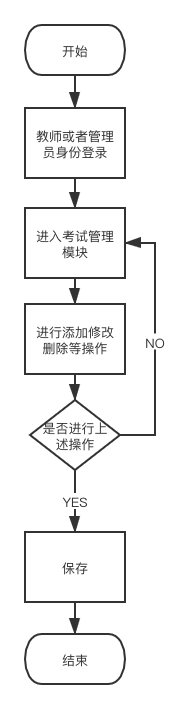
\includegraphics[width=0.3\textwidth,keepaspectratio]{data/chapter-5/examManage.png}
\caption{考试管理模块流程图}
\label{figure:examManage}
\end{figure}
\subsection{试题管理模块}
该模块主要用于试题库的建设和维护,可以对试题进行添加、删除、修改和查询。该模块结构图如图\ref{figure:question}所示。
\begin{figure}[H]
\centering
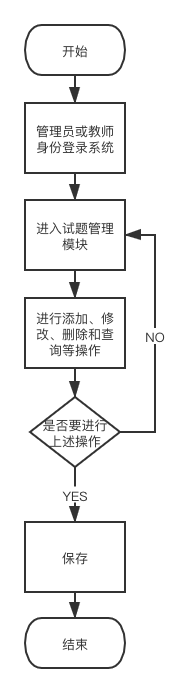
\includegraphics[width=0.3\textwidth,keepaspectratio]{data/chapter-5/question.png}
\caption{试题管理模块流程图}
\label{figure:question}
\end{figure}
\subsection{组卷管理模块}
该模块主要用于提供试卷。可以有教师手工组卷,具体操作如下:进入手工组卷页面,选择相关的科目即可从题库中调出相关题目的列表。
该模块结构图如图\ref{figure:makeup}所示。
\begin{figure}[H]
\centering
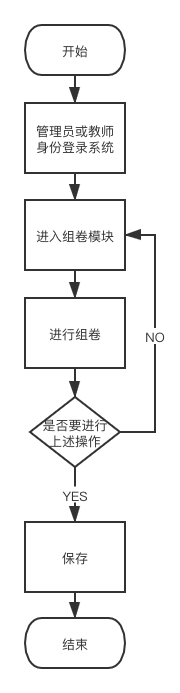
\includegraphics[width=0.2\textwidth,keepaspectratio]{data/chapter-5/makeup.png}
\caption{组卷模块流程图}
\label{figure:makeup}
\end{figure}
\subsection{成绩管理模块}
该模块主要用于查看学生考试的历史记录以及对为批改的主观题进行评分和评语。
\subsection{个人信息管理模块}
该模块主要用于用户对自己信息进行修改。该模块结构图如图\ref{figure:information}所示。
\begin{figure}[H]
\centering
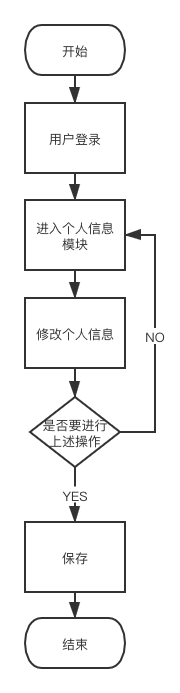
\includegraphics[width=0.3\textwidth,keepaspectratio]{data/chapter-5/information.png}
\caption{个人信息管理模块}
\label{figure:information}
\end{figure}

\section{管理员子系统的具体实现}
\subsection{登录}
\begin{enumerate}
	\item[] \textbf{功能描述:}通过管理员的用户名和密码进行登录。
	\item[] \textbf{功能页面:}如图\ref{figure:denglu}所示 \\
		\begin{figure}[H]
			\centering
			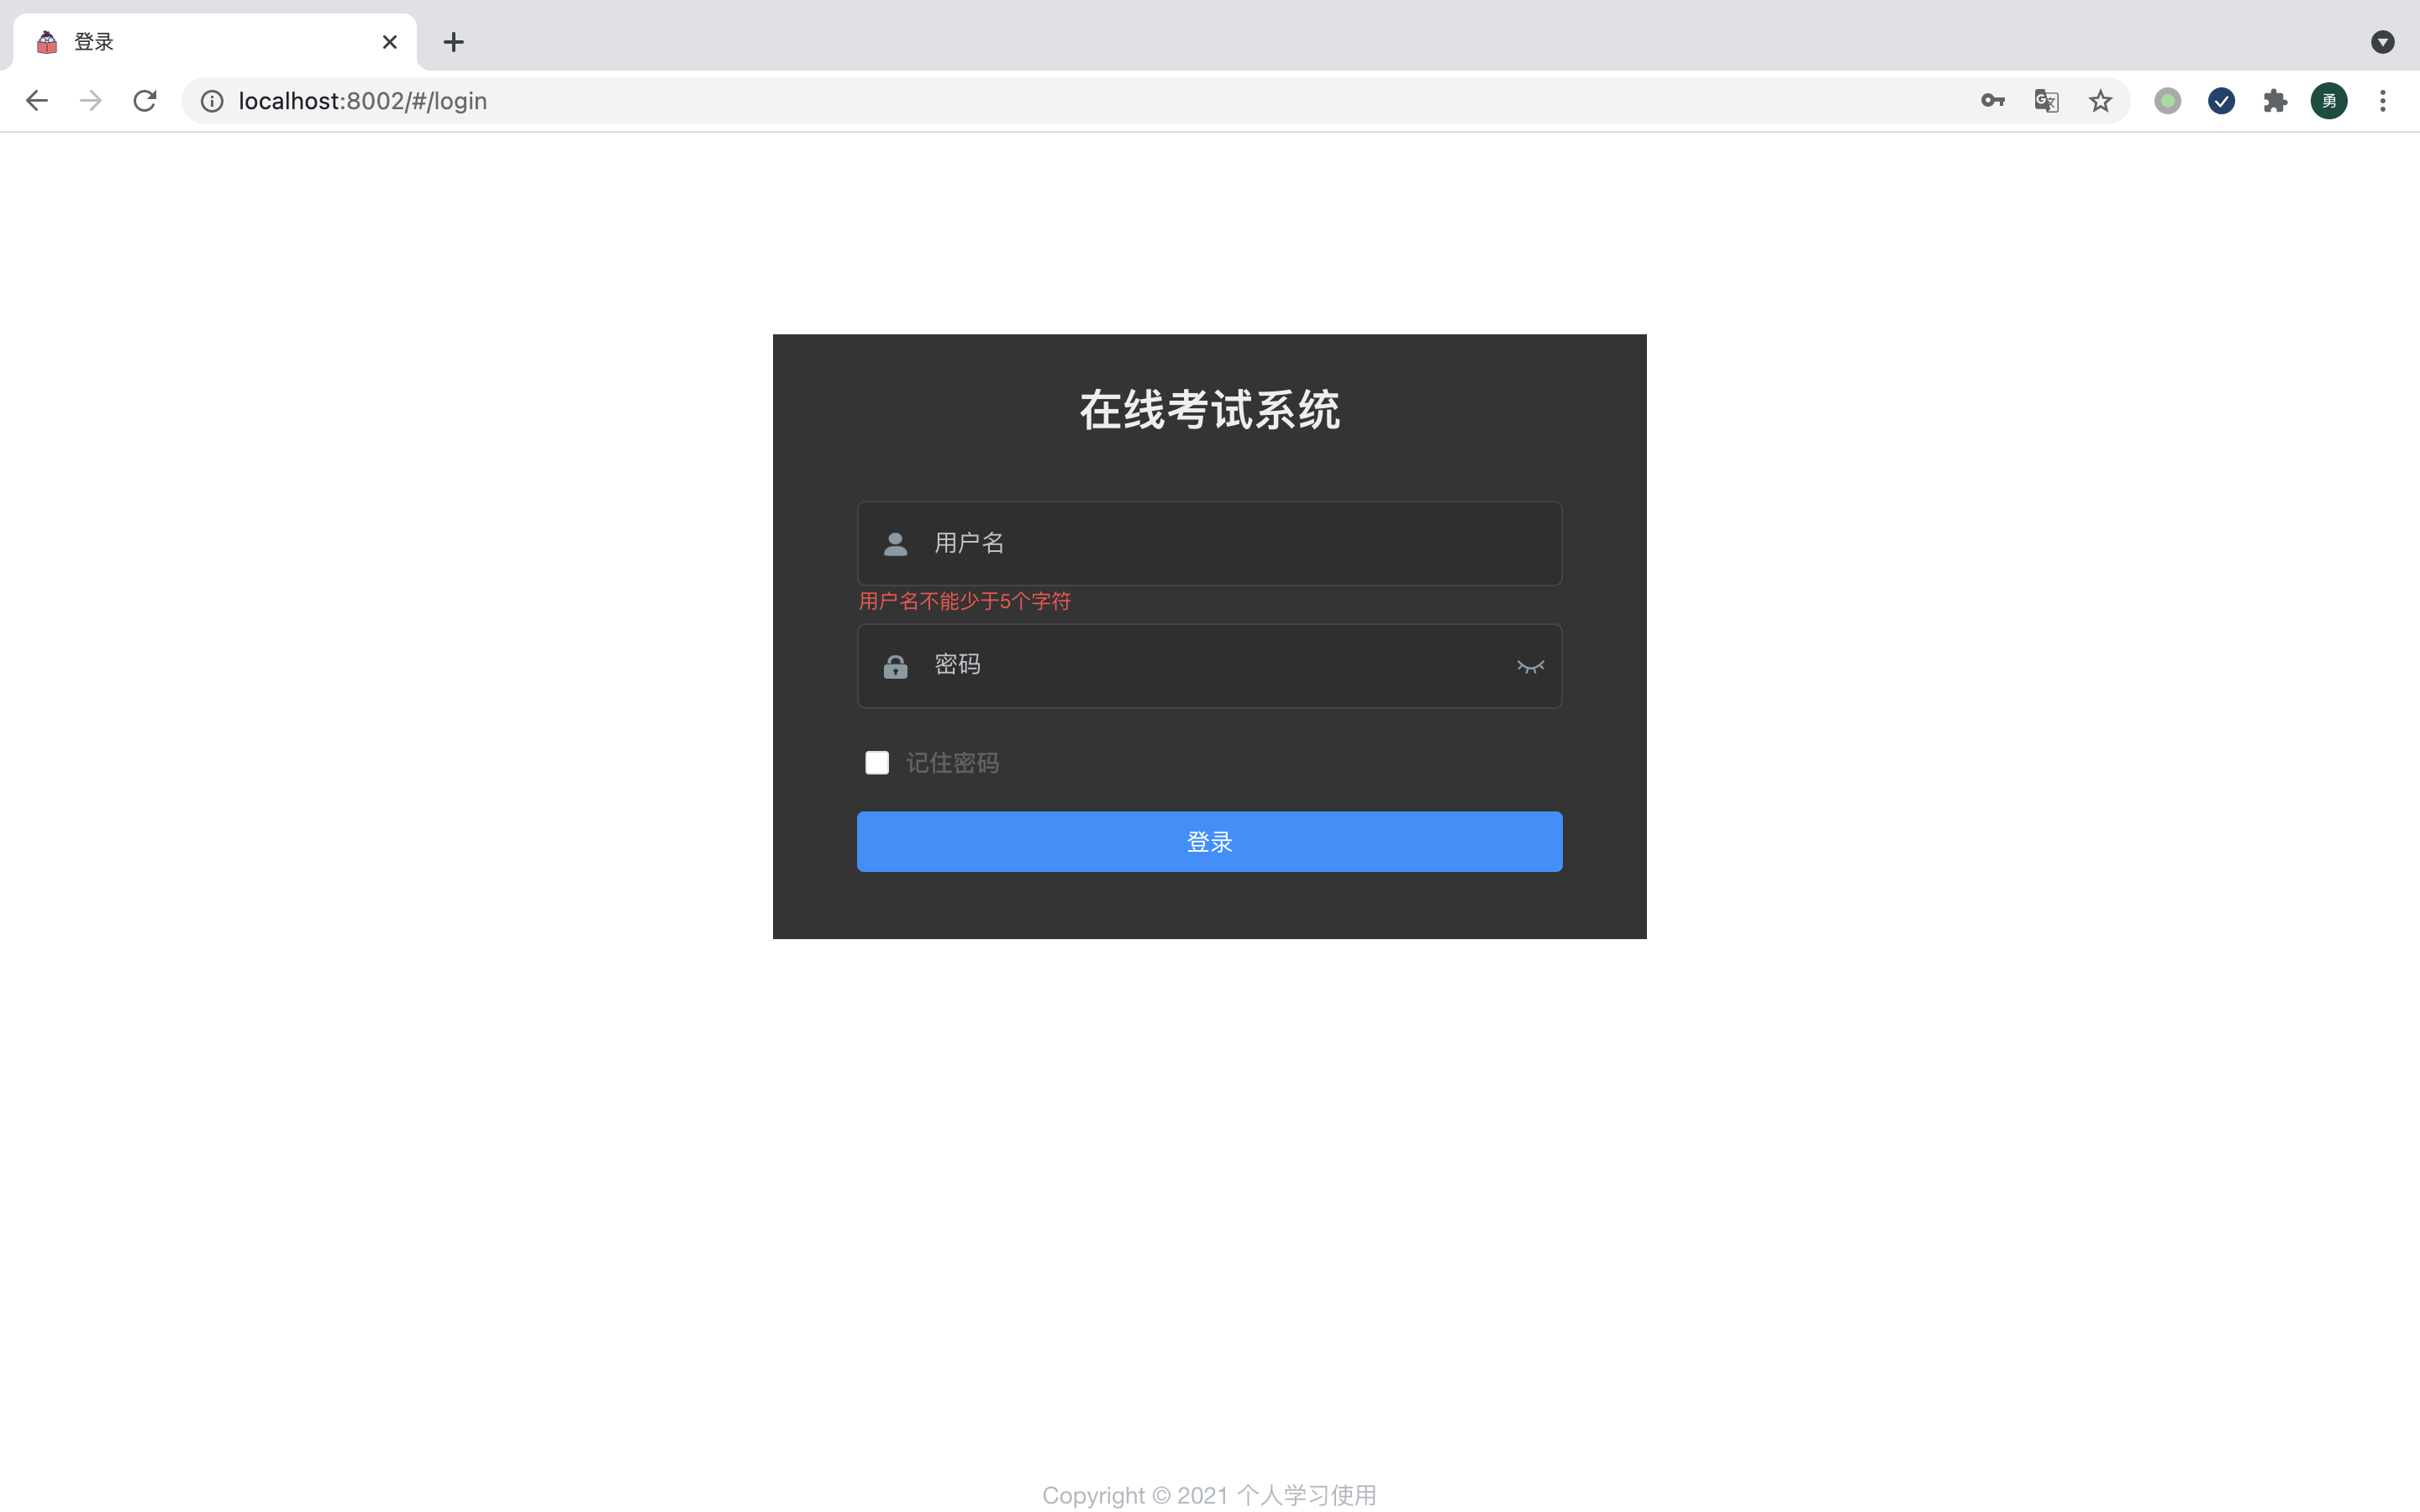
\includegraphics[width=1.0\textwidth,keepaspectratio]{data/chapter-5/denglu.png}
			\caption{登录页面}
			\label{figure:denglu}
		\end{figure}
\end{enumerate}

\subsection{主页}
\begin{enumerate}
	\item[] \textbf{功能描述:}管理员界面的仪表盘,显示常用数据。
	\item[] \textbf{功能页面:}如图\ref{figure:zhuye}所示 \\
		\begin{figure}[H]
			\centering
			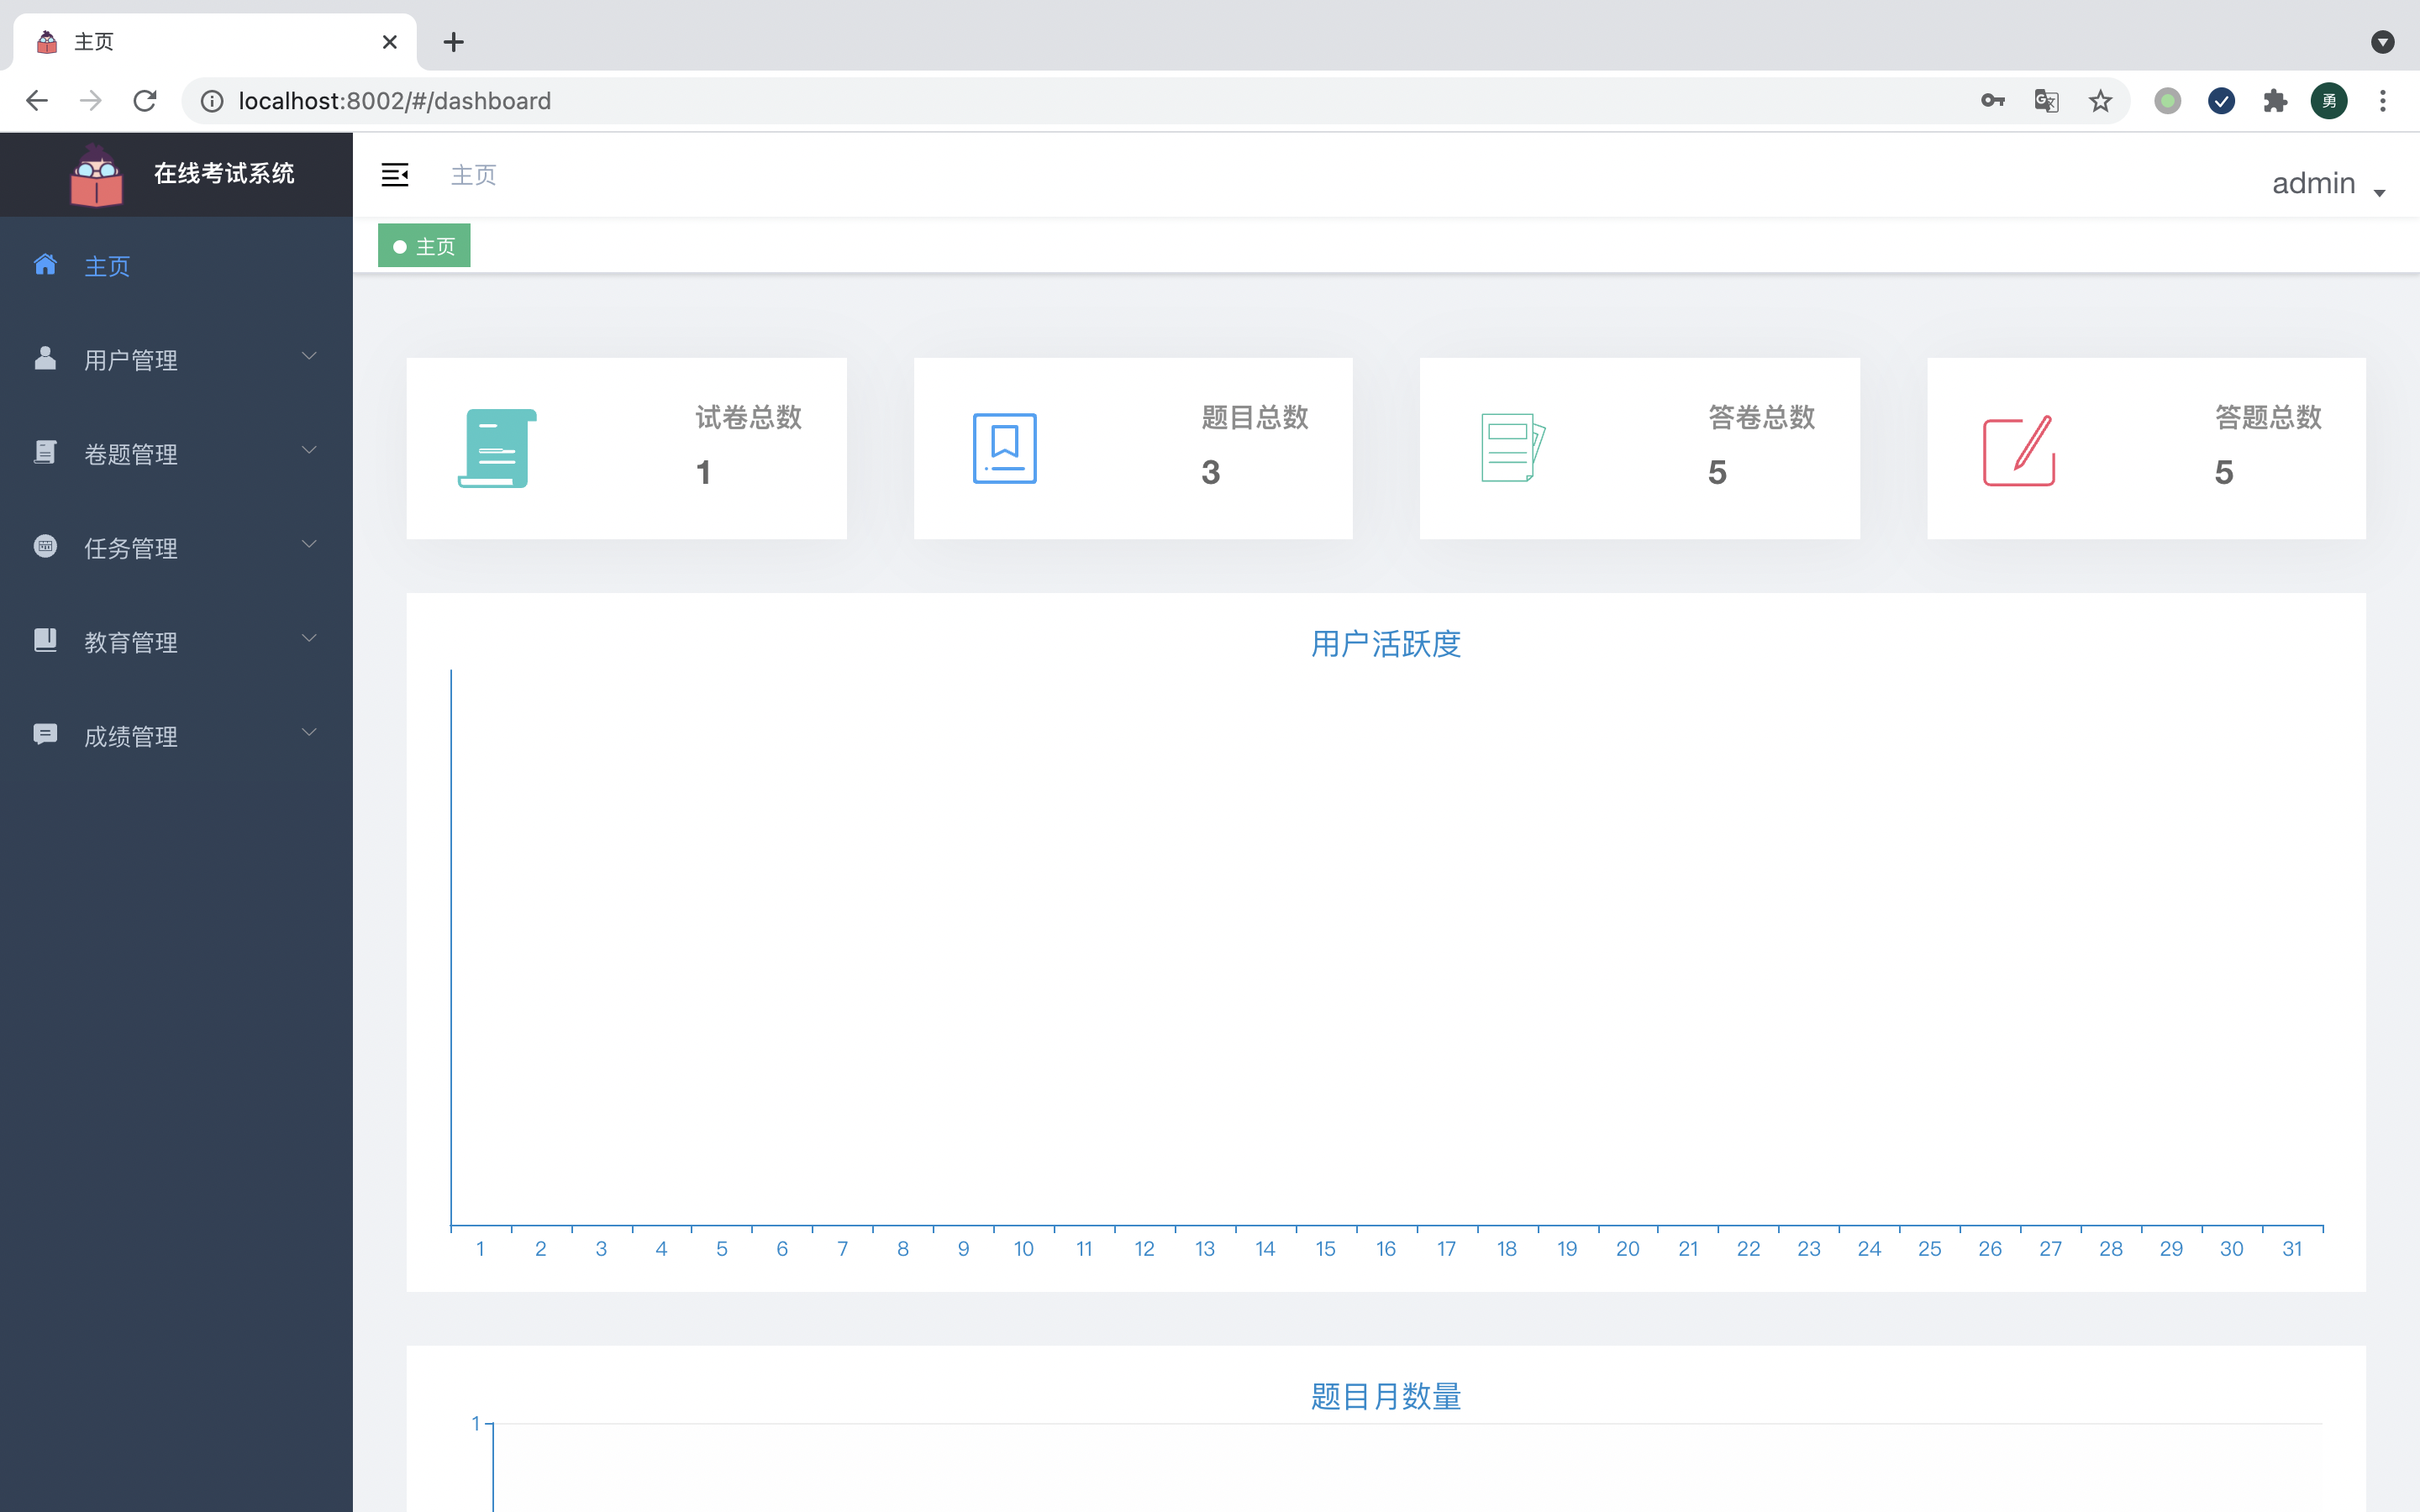
\includegraphics[width=1.0\textwidth,keepaspectratio]{data/chapter-5/zhuye.png}
			\caption{管理员主页}
			\label{figure:zhuye}
		\end{figure}
\end{enumerate}

\subsection{用户管理}
\begin{enumerate}
	\item[] \textbf{功能描述:}用户管理功能界面,可以对所有用户进行信息的修改,同时可以添加或删除用户。
	\item[] \textbf{功能页面:}如图\ref{figure:yonghu}所示 \\
		\begin{figure}[H]
			\centering
			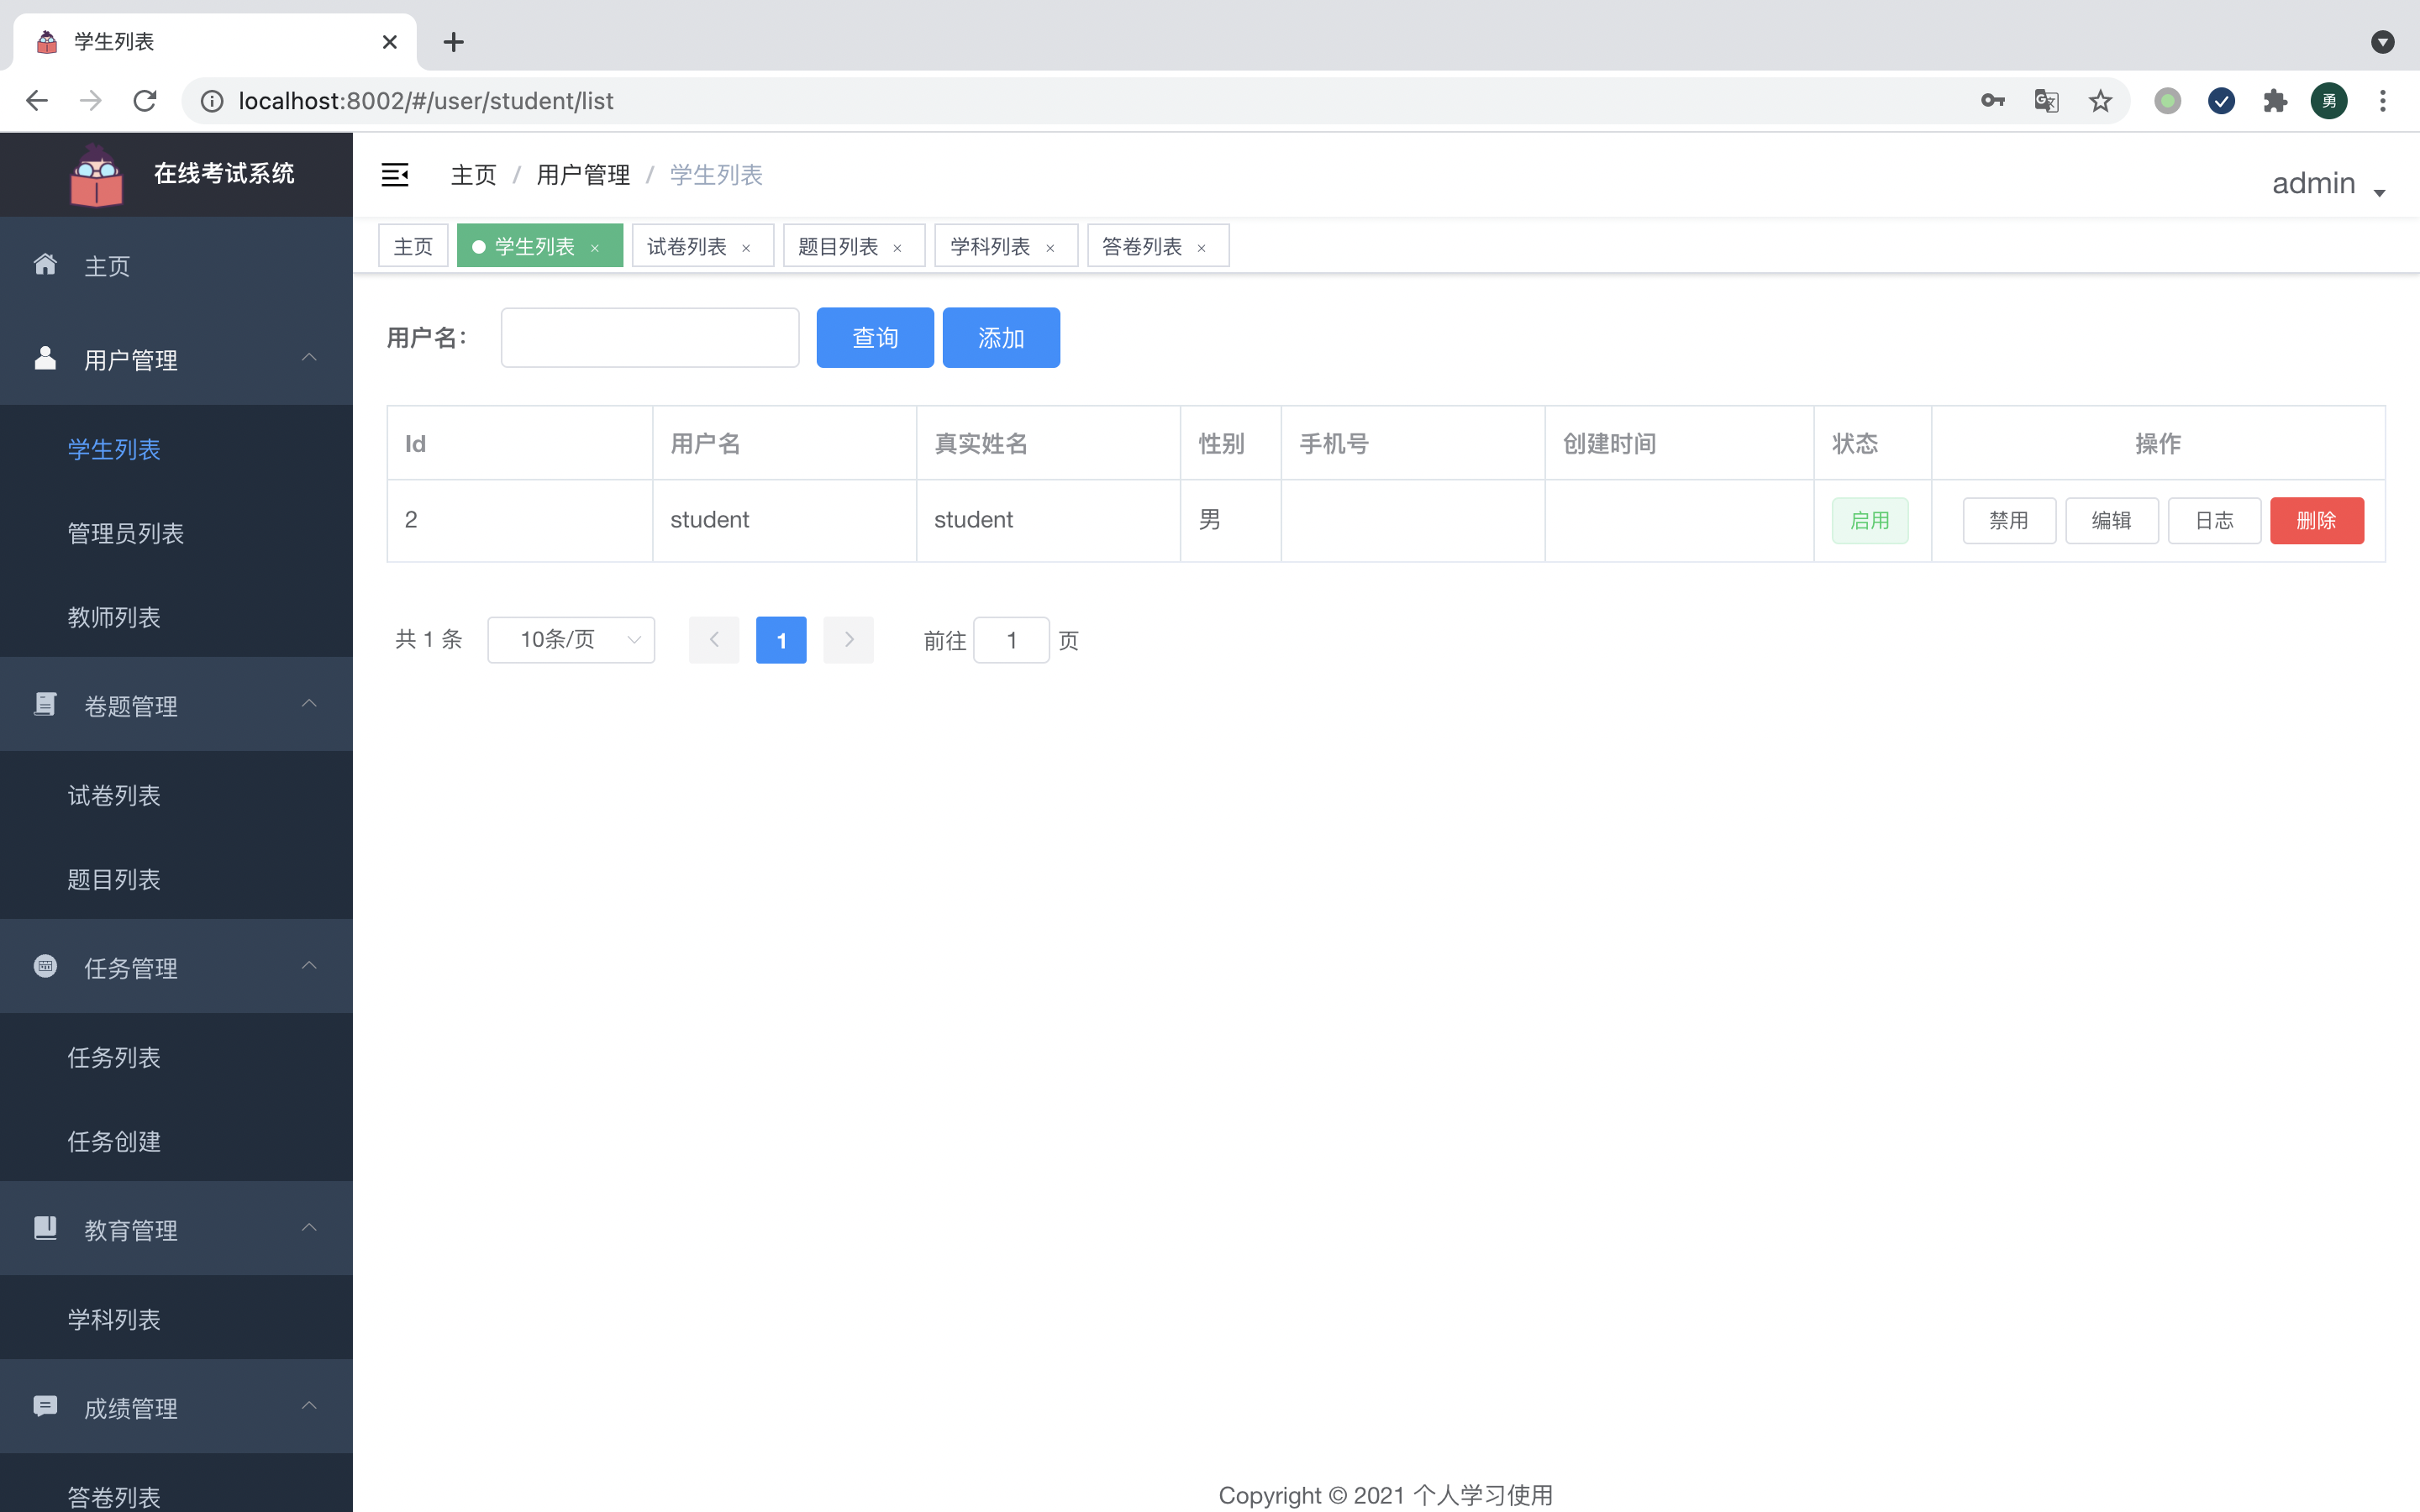
\includegraphics[width=1.0\textwidth,keepaspectratio]{data/chapter-5/yonghu.png}
			\caption{用户管理}
			\label{figure:yonghu}
		\end{figure}
\end{enumerate}

\subsection{试卷管理}
\begin{enumerate}
	\item[] \textbf{功能描述:}试卷管理功能界面,可以对所有试卷进行内容的修改,同时可以添加或删除试卷。
	\item[] \textbf{功能页面:}如图\ref{figure:shijuan}所示 \\
		\begin{figure}[H]
			\centering
			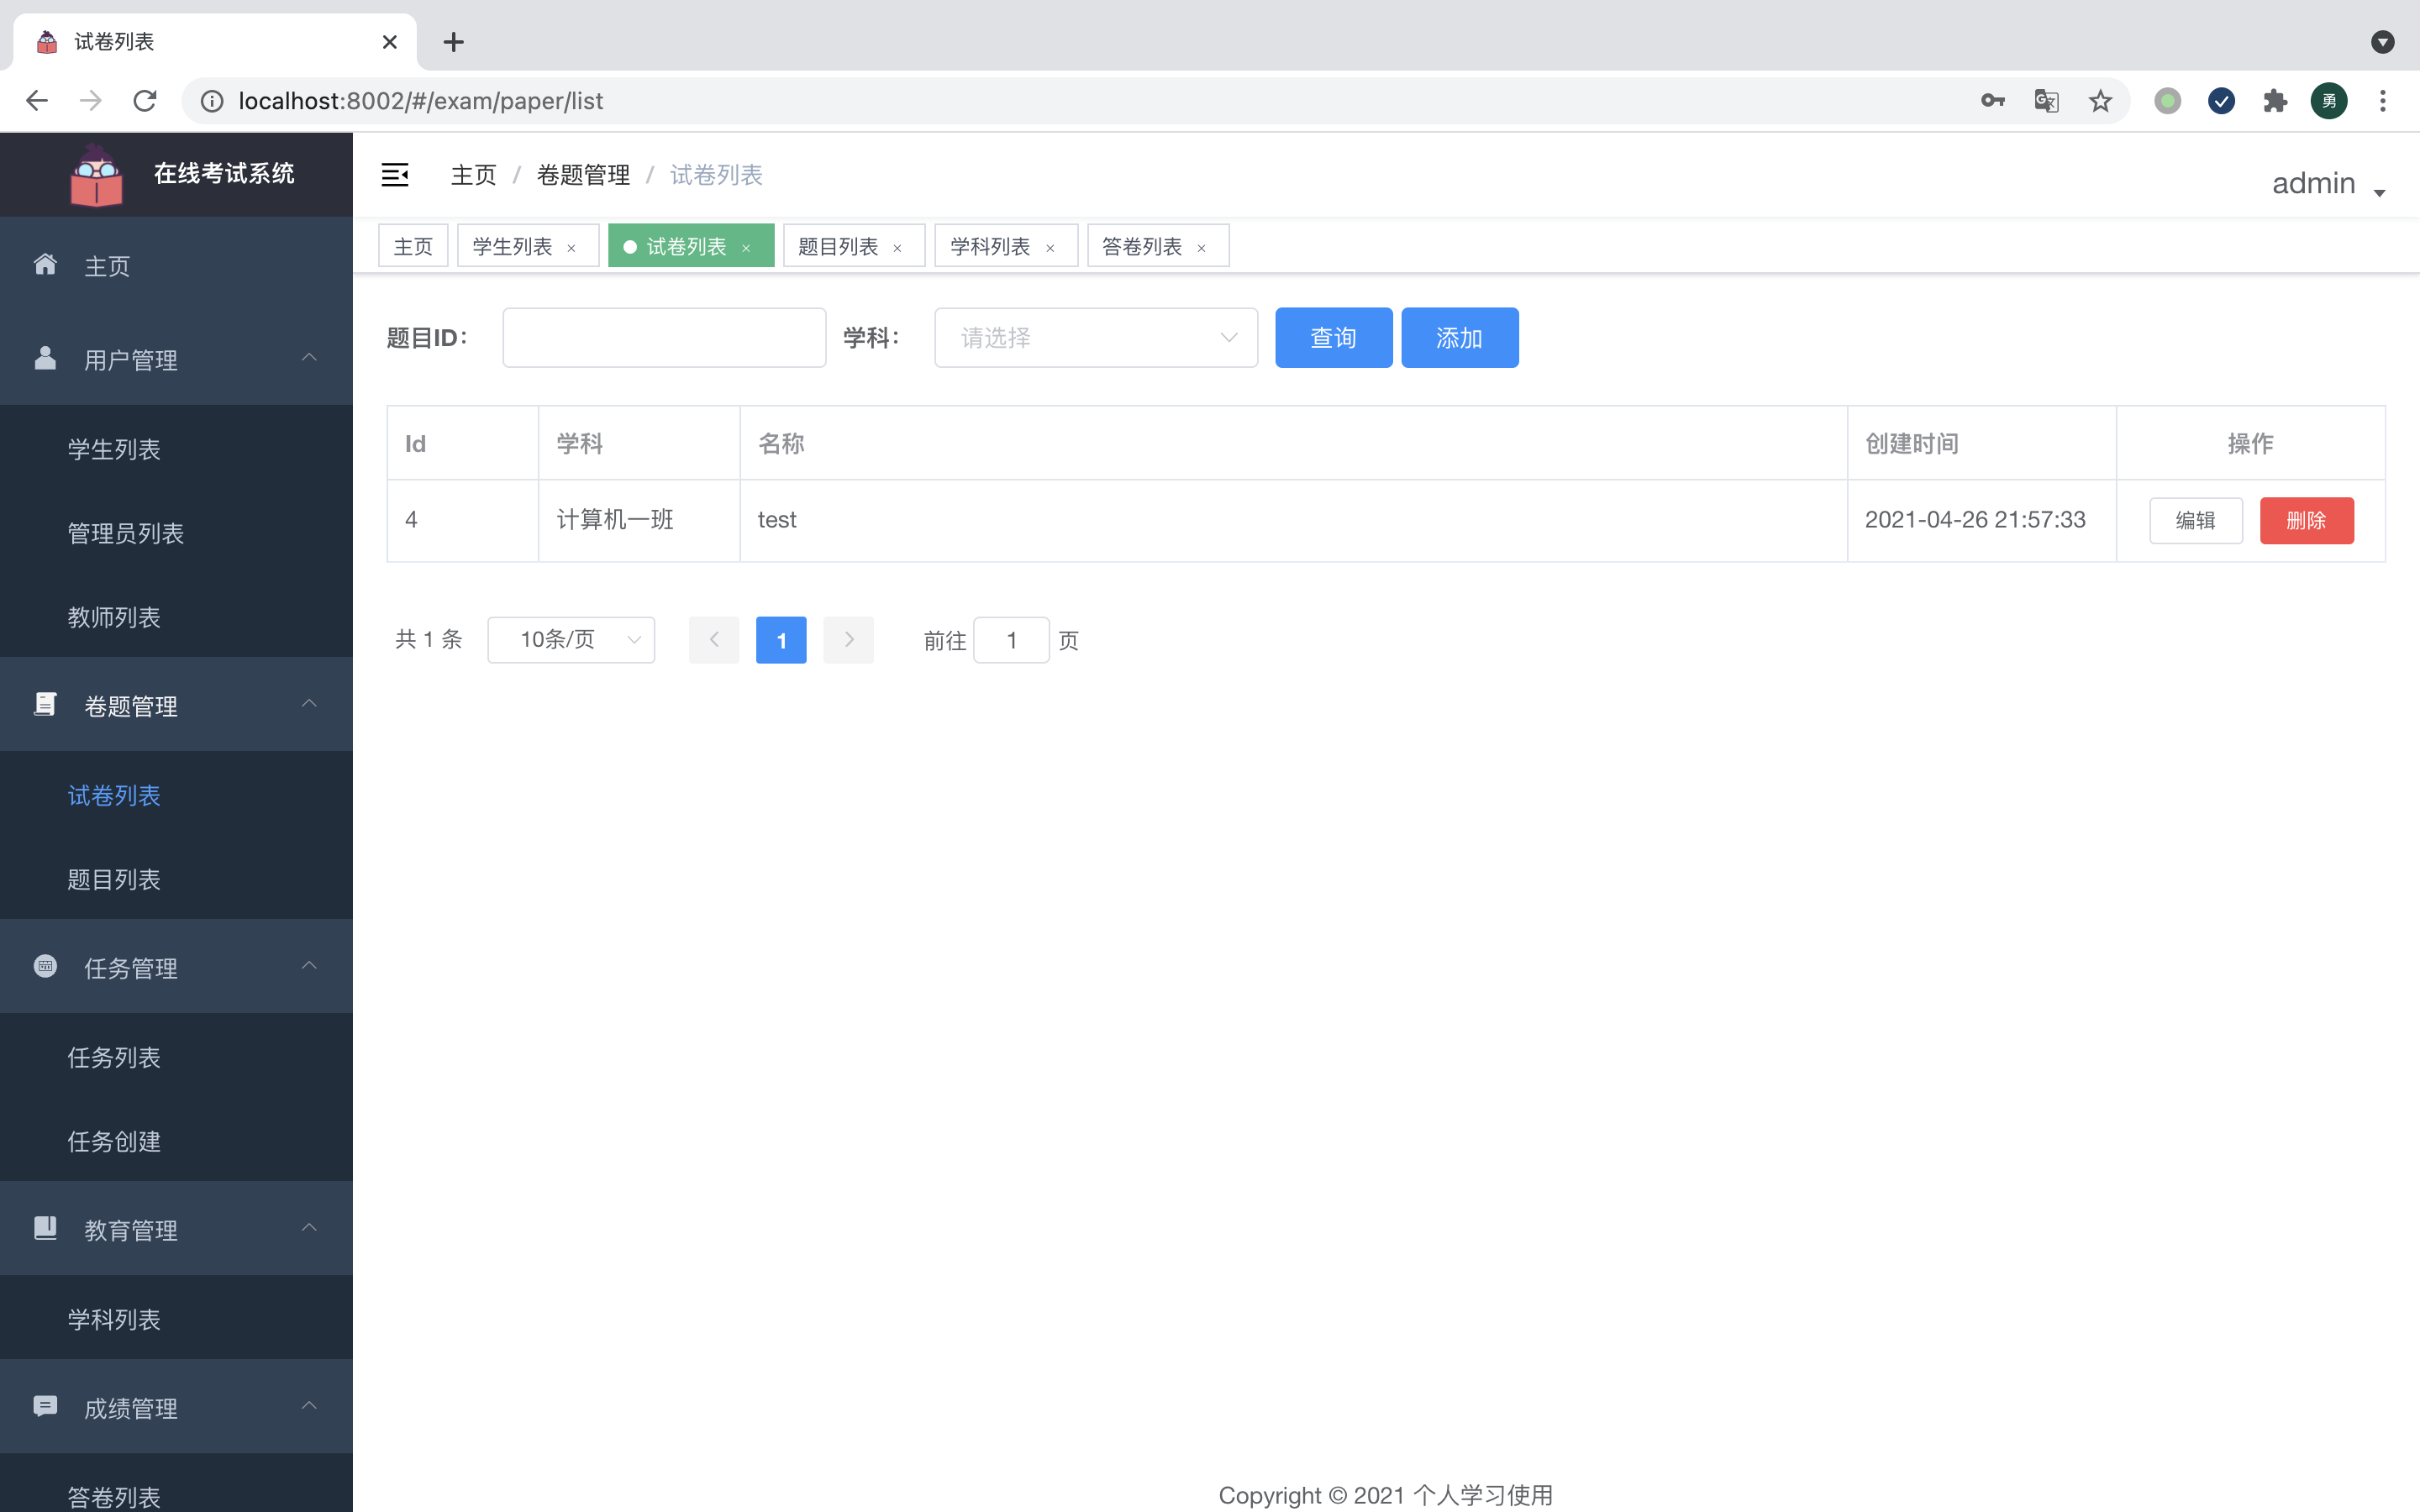
\includegraphics[width=1.0\textwidth,keepaspectratio]{data/chapter-5/shijuan.png}
			\caption{试卷管理}
			\label{figure:shijuan}
		\end{figure}
\end{enumerate}

\subsection{试题管理}
\begin{enumerate}
	\item[] \textbf{功能描述:}试题管理功能界面,可以对所有试题进行内容的修改,同时可以添加或删除试题。
	\item[] \textbf{功能页面:}如图\ref{figure:timu}所示 \\
		\begin{figure}[H]
			\centering
			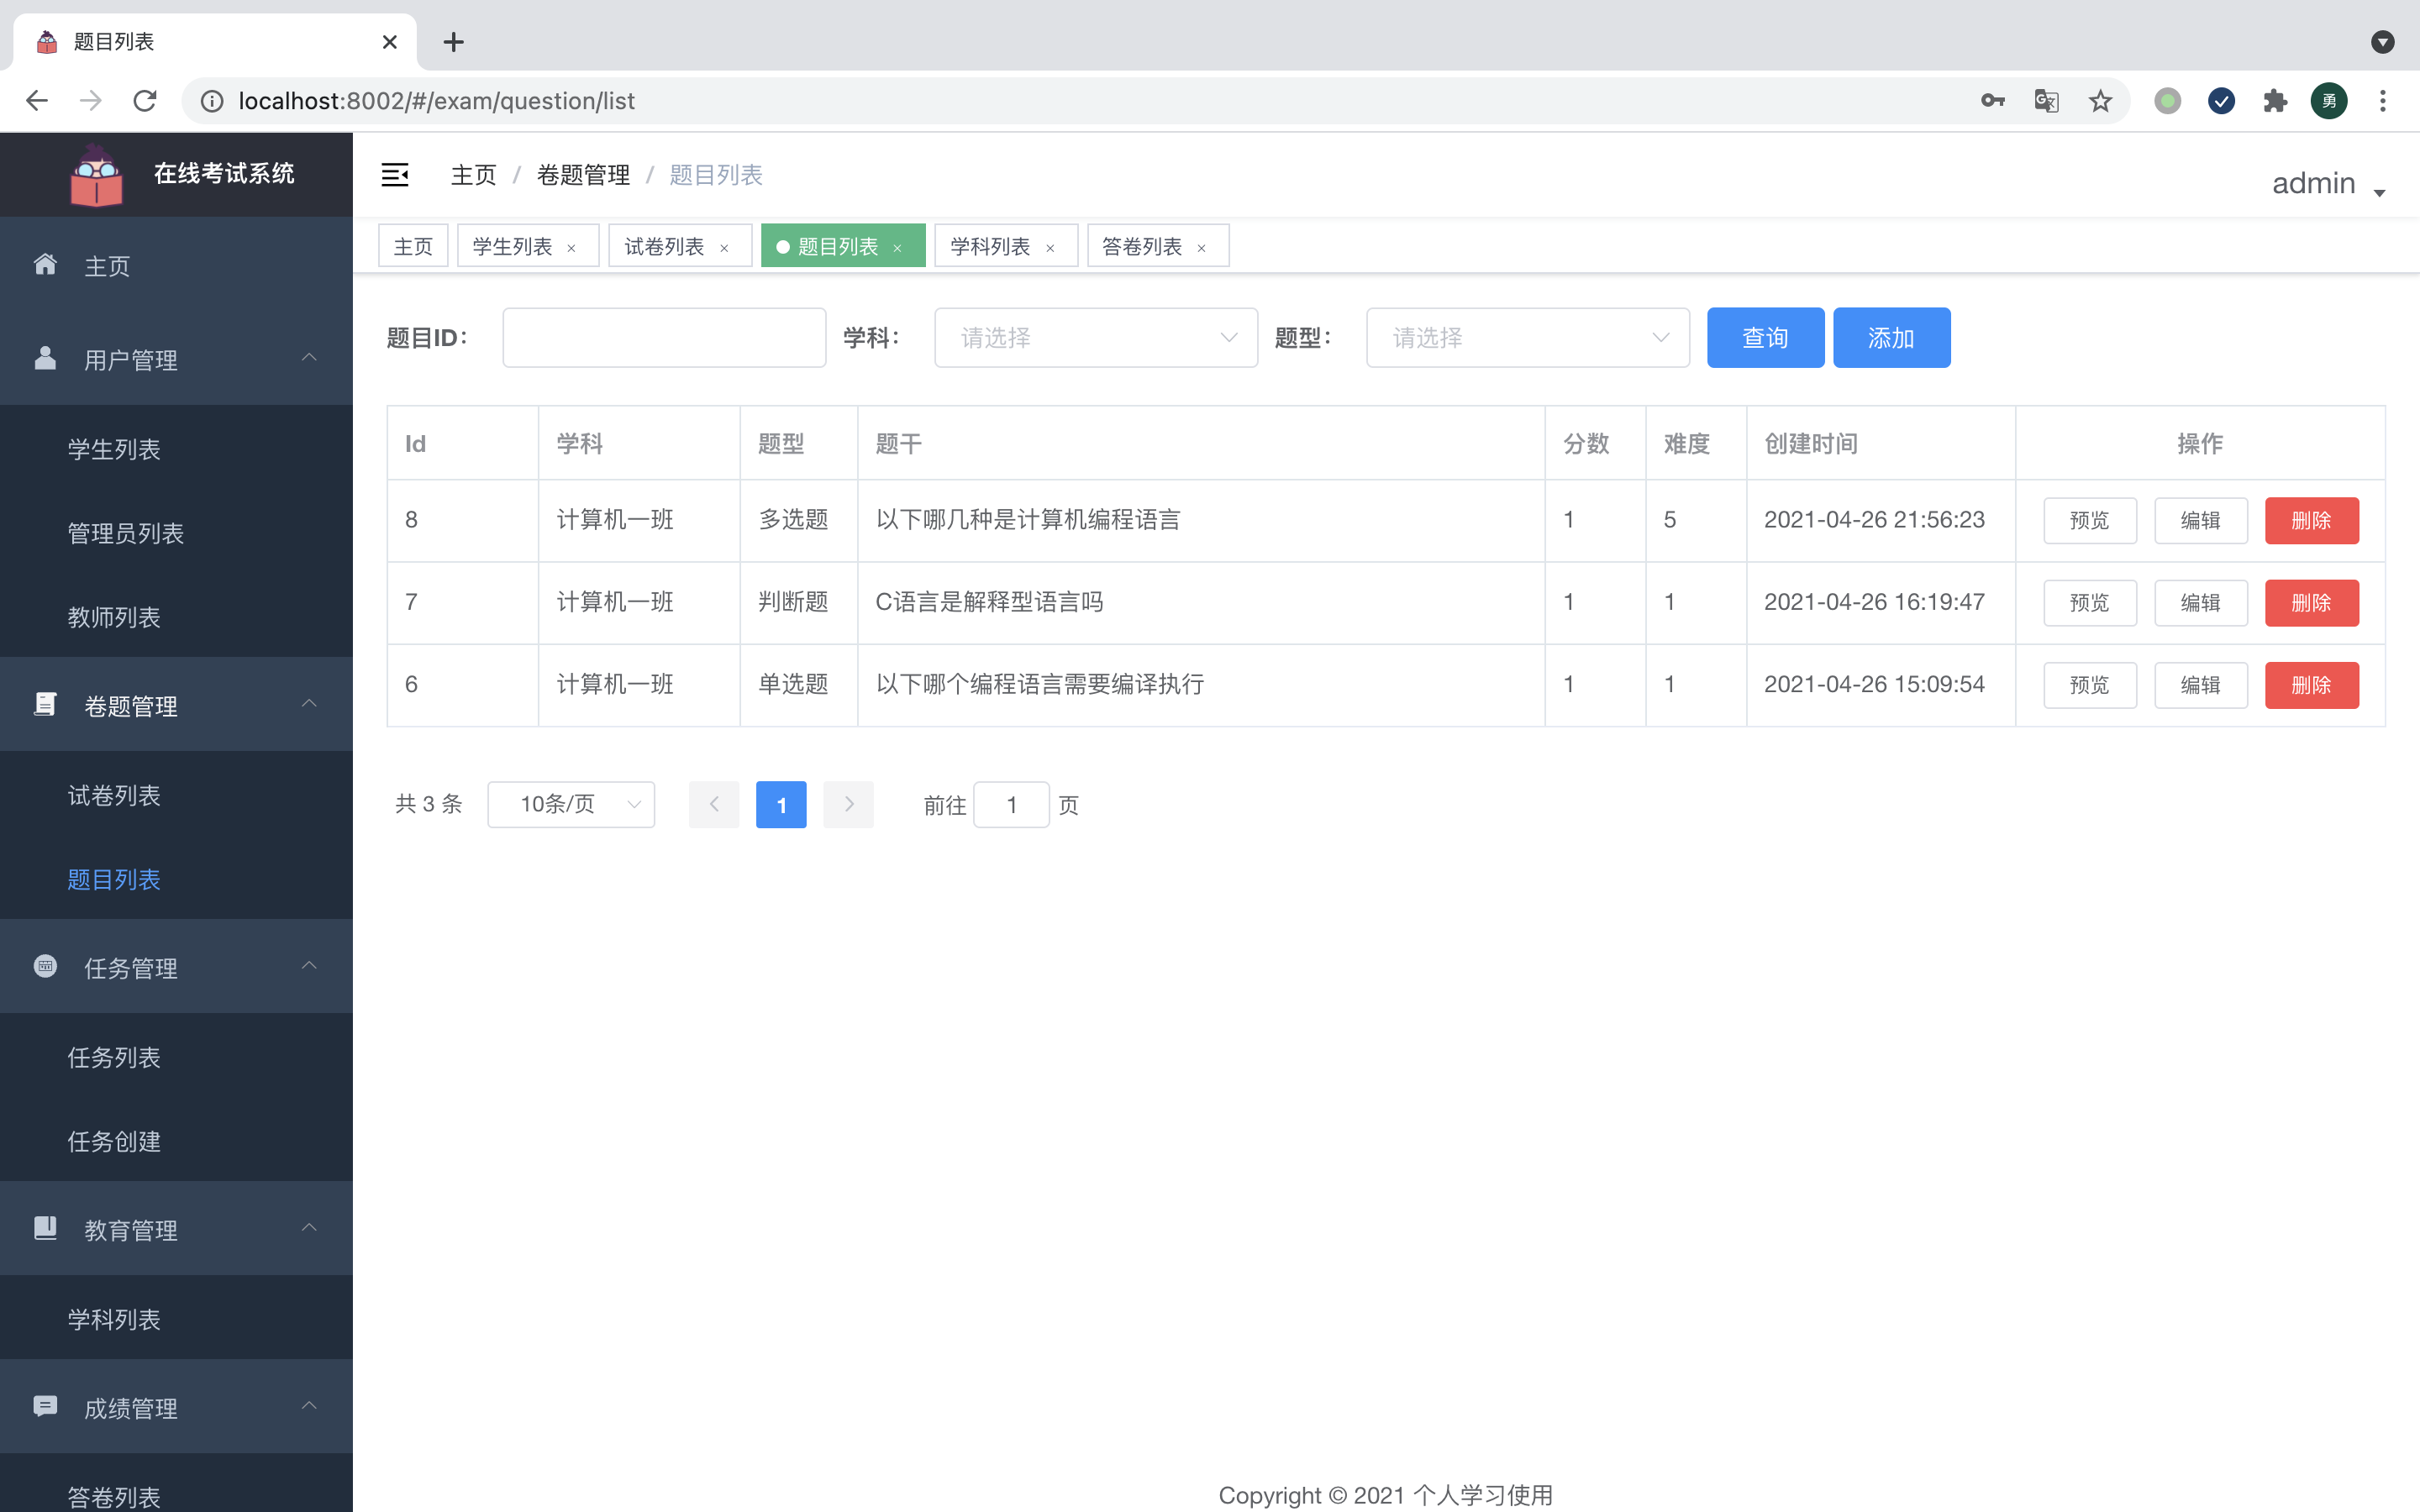
\includegraphics[width=1.0\textwidth,keepaspectratio]{data/chapter-5/timu.png}
			\caption{试题管理}
			\label{figure:timu}
		\end{figure}
\end{enumerate}

\subsection{班级管理}
\begin{enumerate}
	\item[] \textbf{功能描述:}班级管理功能界面,可以对所有班级进行信息的修改,同时可以添加或删除班级。
	\item[] \textbf{功能页面:}如图\ref{figure:xueke}所示 \\
		\begin{figure}[H]
			\centering
			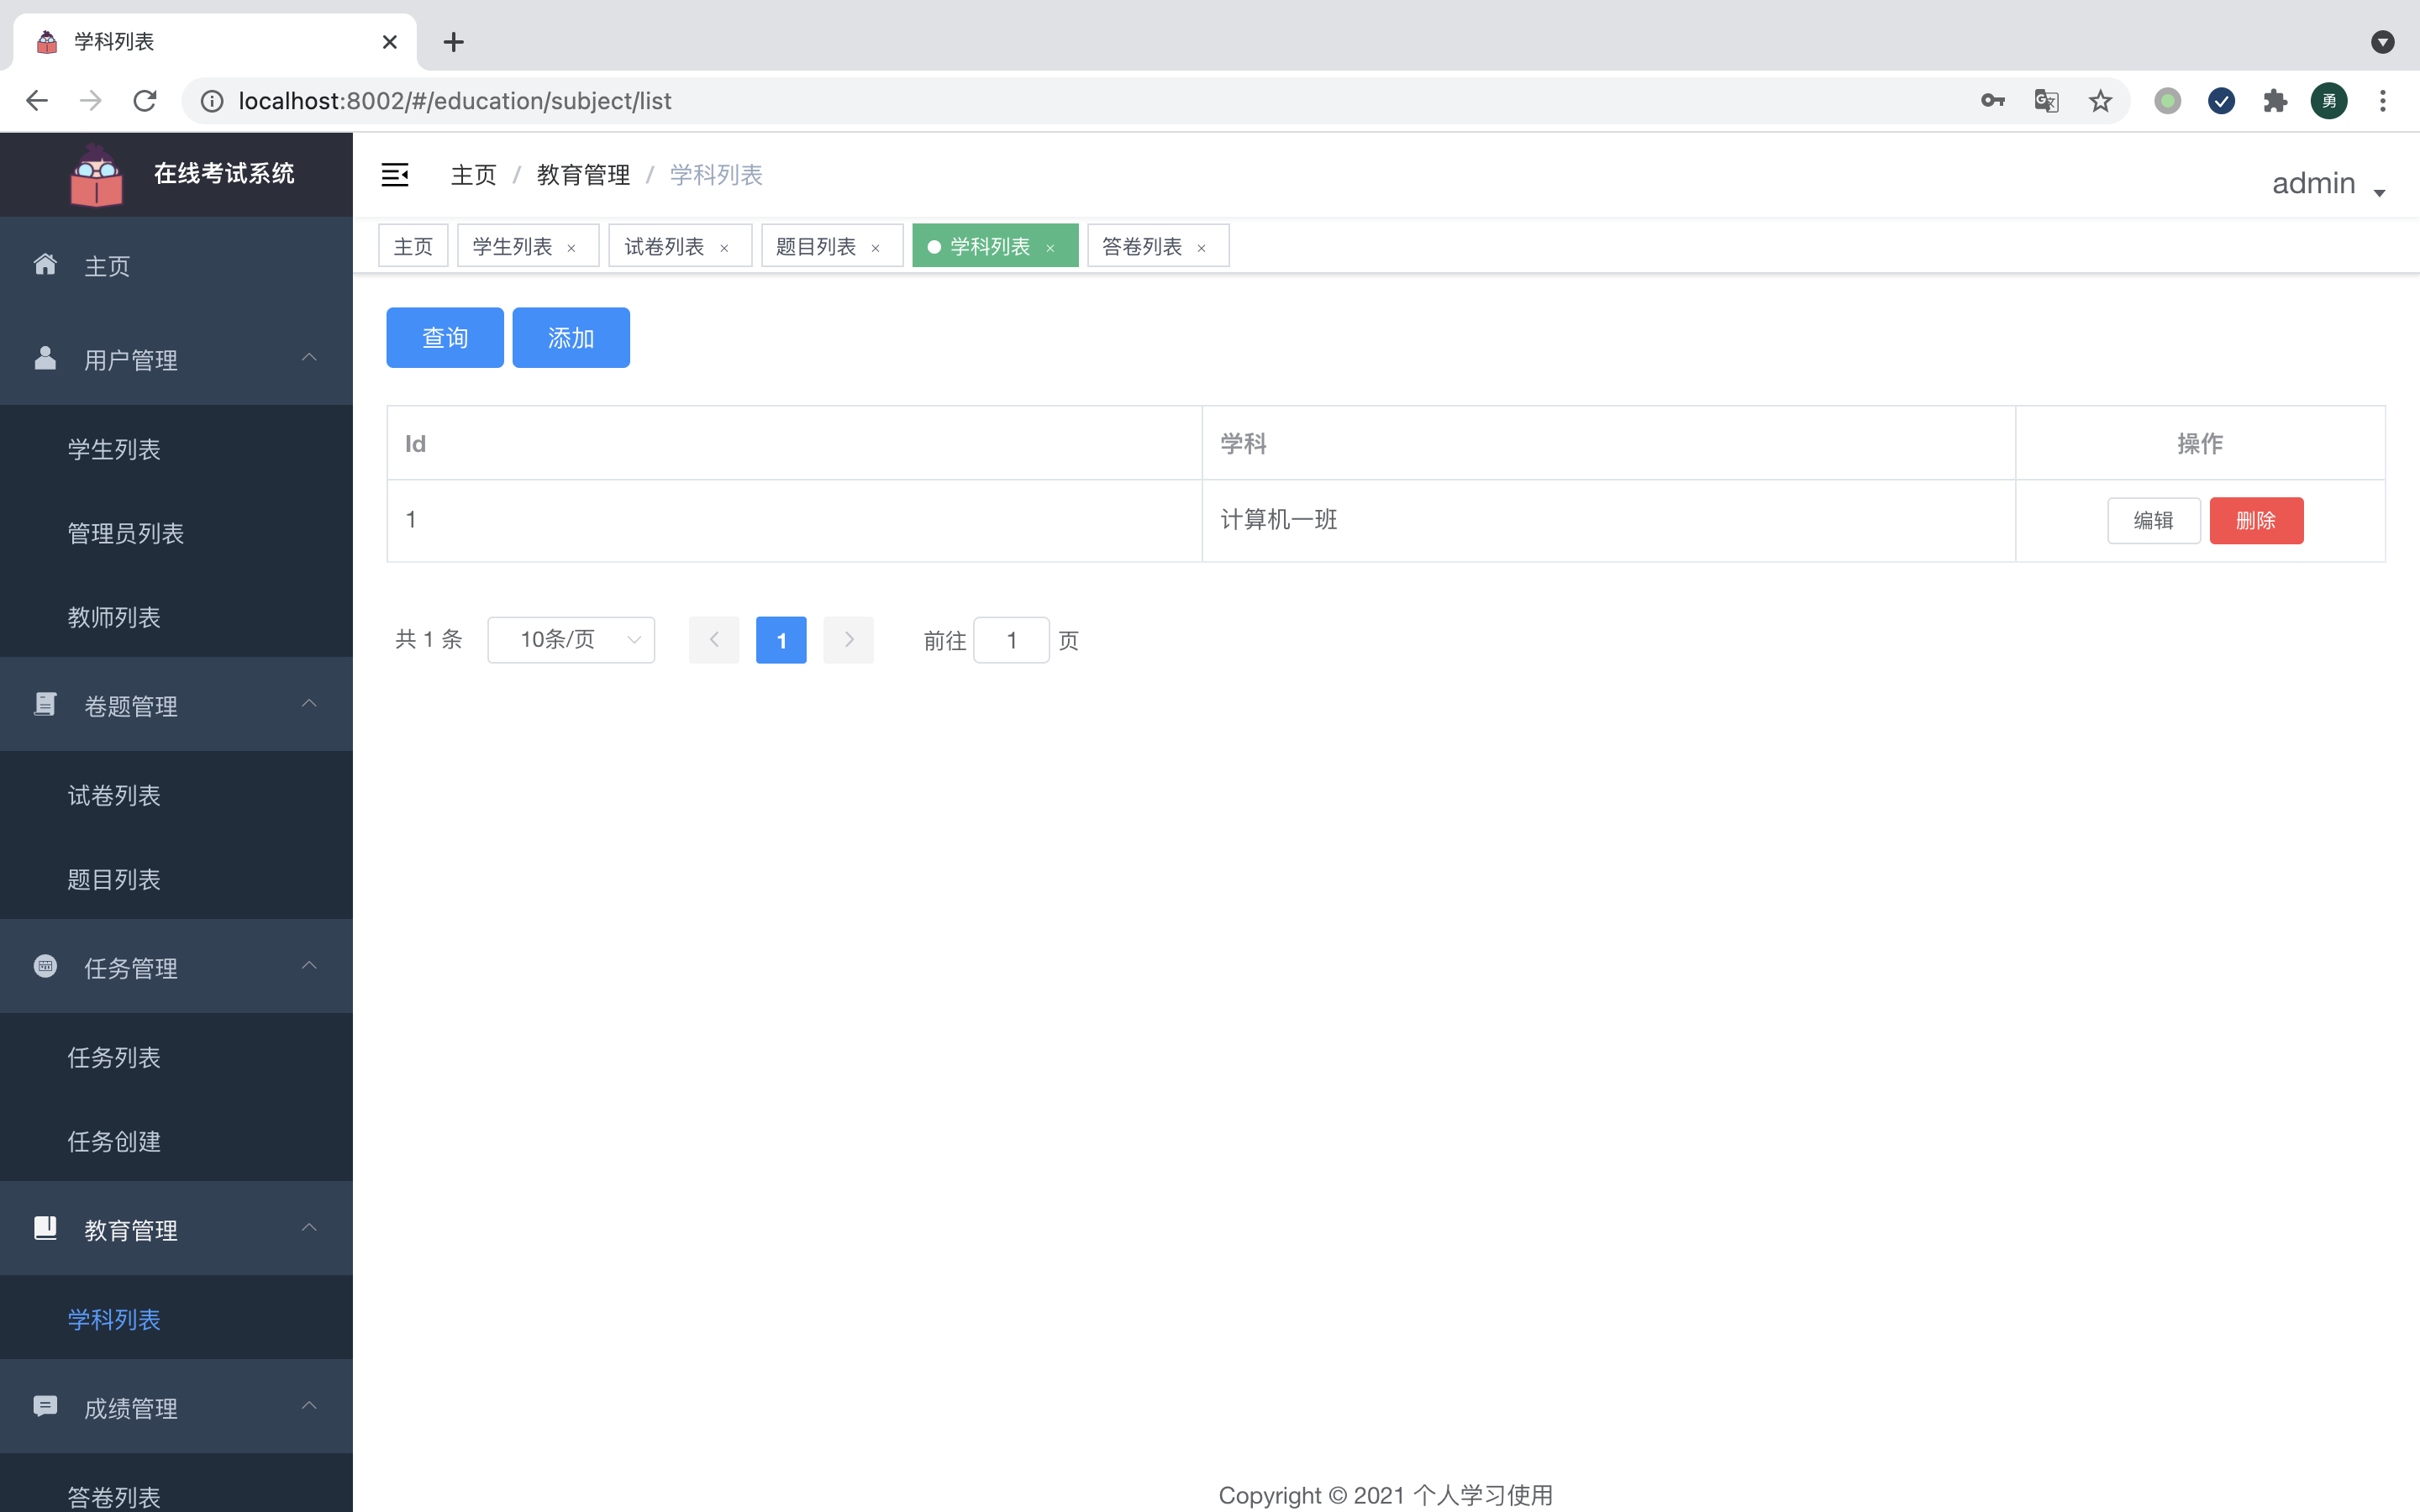
\includegraphics[width=1.0\textwidth,keepaspectratio]{data/chapter-5/xueke.png}
			\caption{班级管理}
			\label{figure:xueke}
		\end{figure}
\end{enumerate}

\subsection{教育管理}
\begin{enumerate}
	\item[] \textbf{功能描述:}教育管理功能界面,试卷的批改和历史试卷的查看。
	\item[] \textbf{功能页面:}如图\ref{figure:dajuan}所示 \\
		\begin{figure}[H]
			\centering
			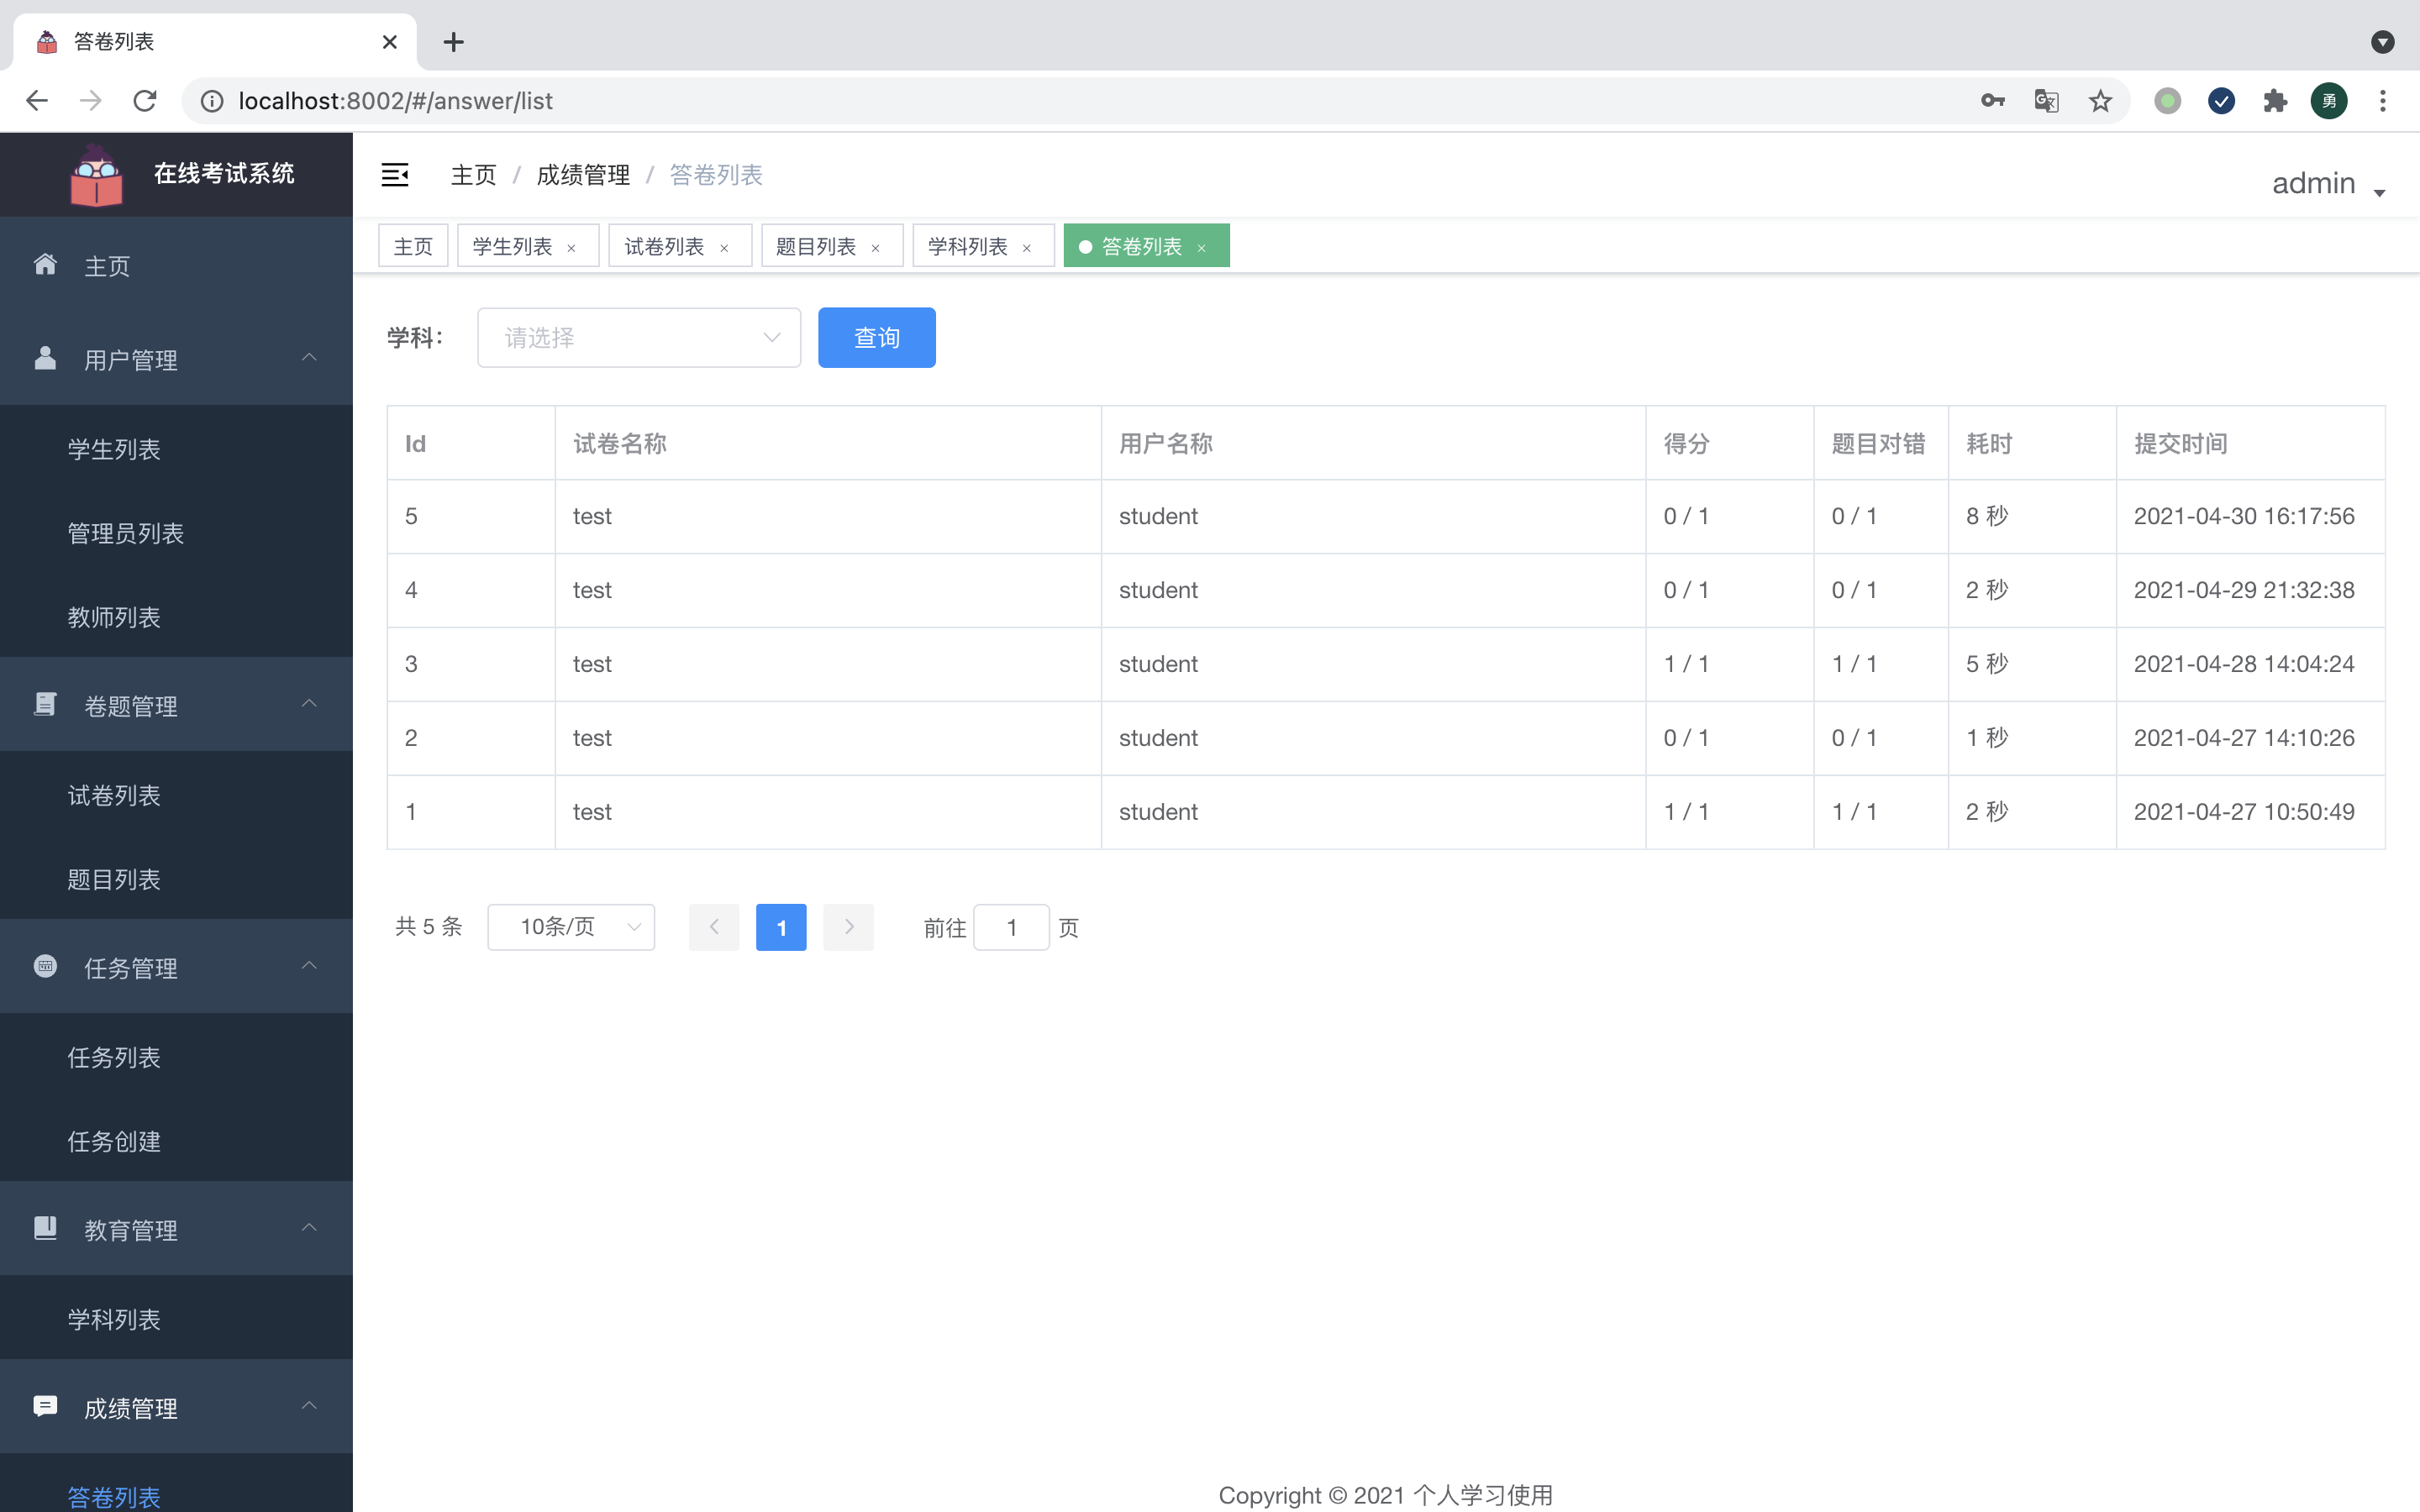
\includegraphics[width=1.0\textwidth,keepaspectratio]{data/chapter-5/dajuan.png}
			\caption{教育管理}
			\label{figure:dajuan}
		\end{figure}
\end{enumerate}

\section{老师子系统的具体实现}
老师子系统和管理员子系统的页面和逻辑大致相同,区别在于老师管理的对象为学生而不是全部用户,这里就不一一列出了。

\section{学生子系统的具体实现}
\subsection{学生登录}
\begin{enumerate}
	\item[] \textbf{功能描述:}学生登录界面,学生通过用户名和密码进行登录。
	\item[] \textbf{功能页面:}如图\ref{figure:sdenglu}所示 \\
		\begin{figure}[H]
			\centering
			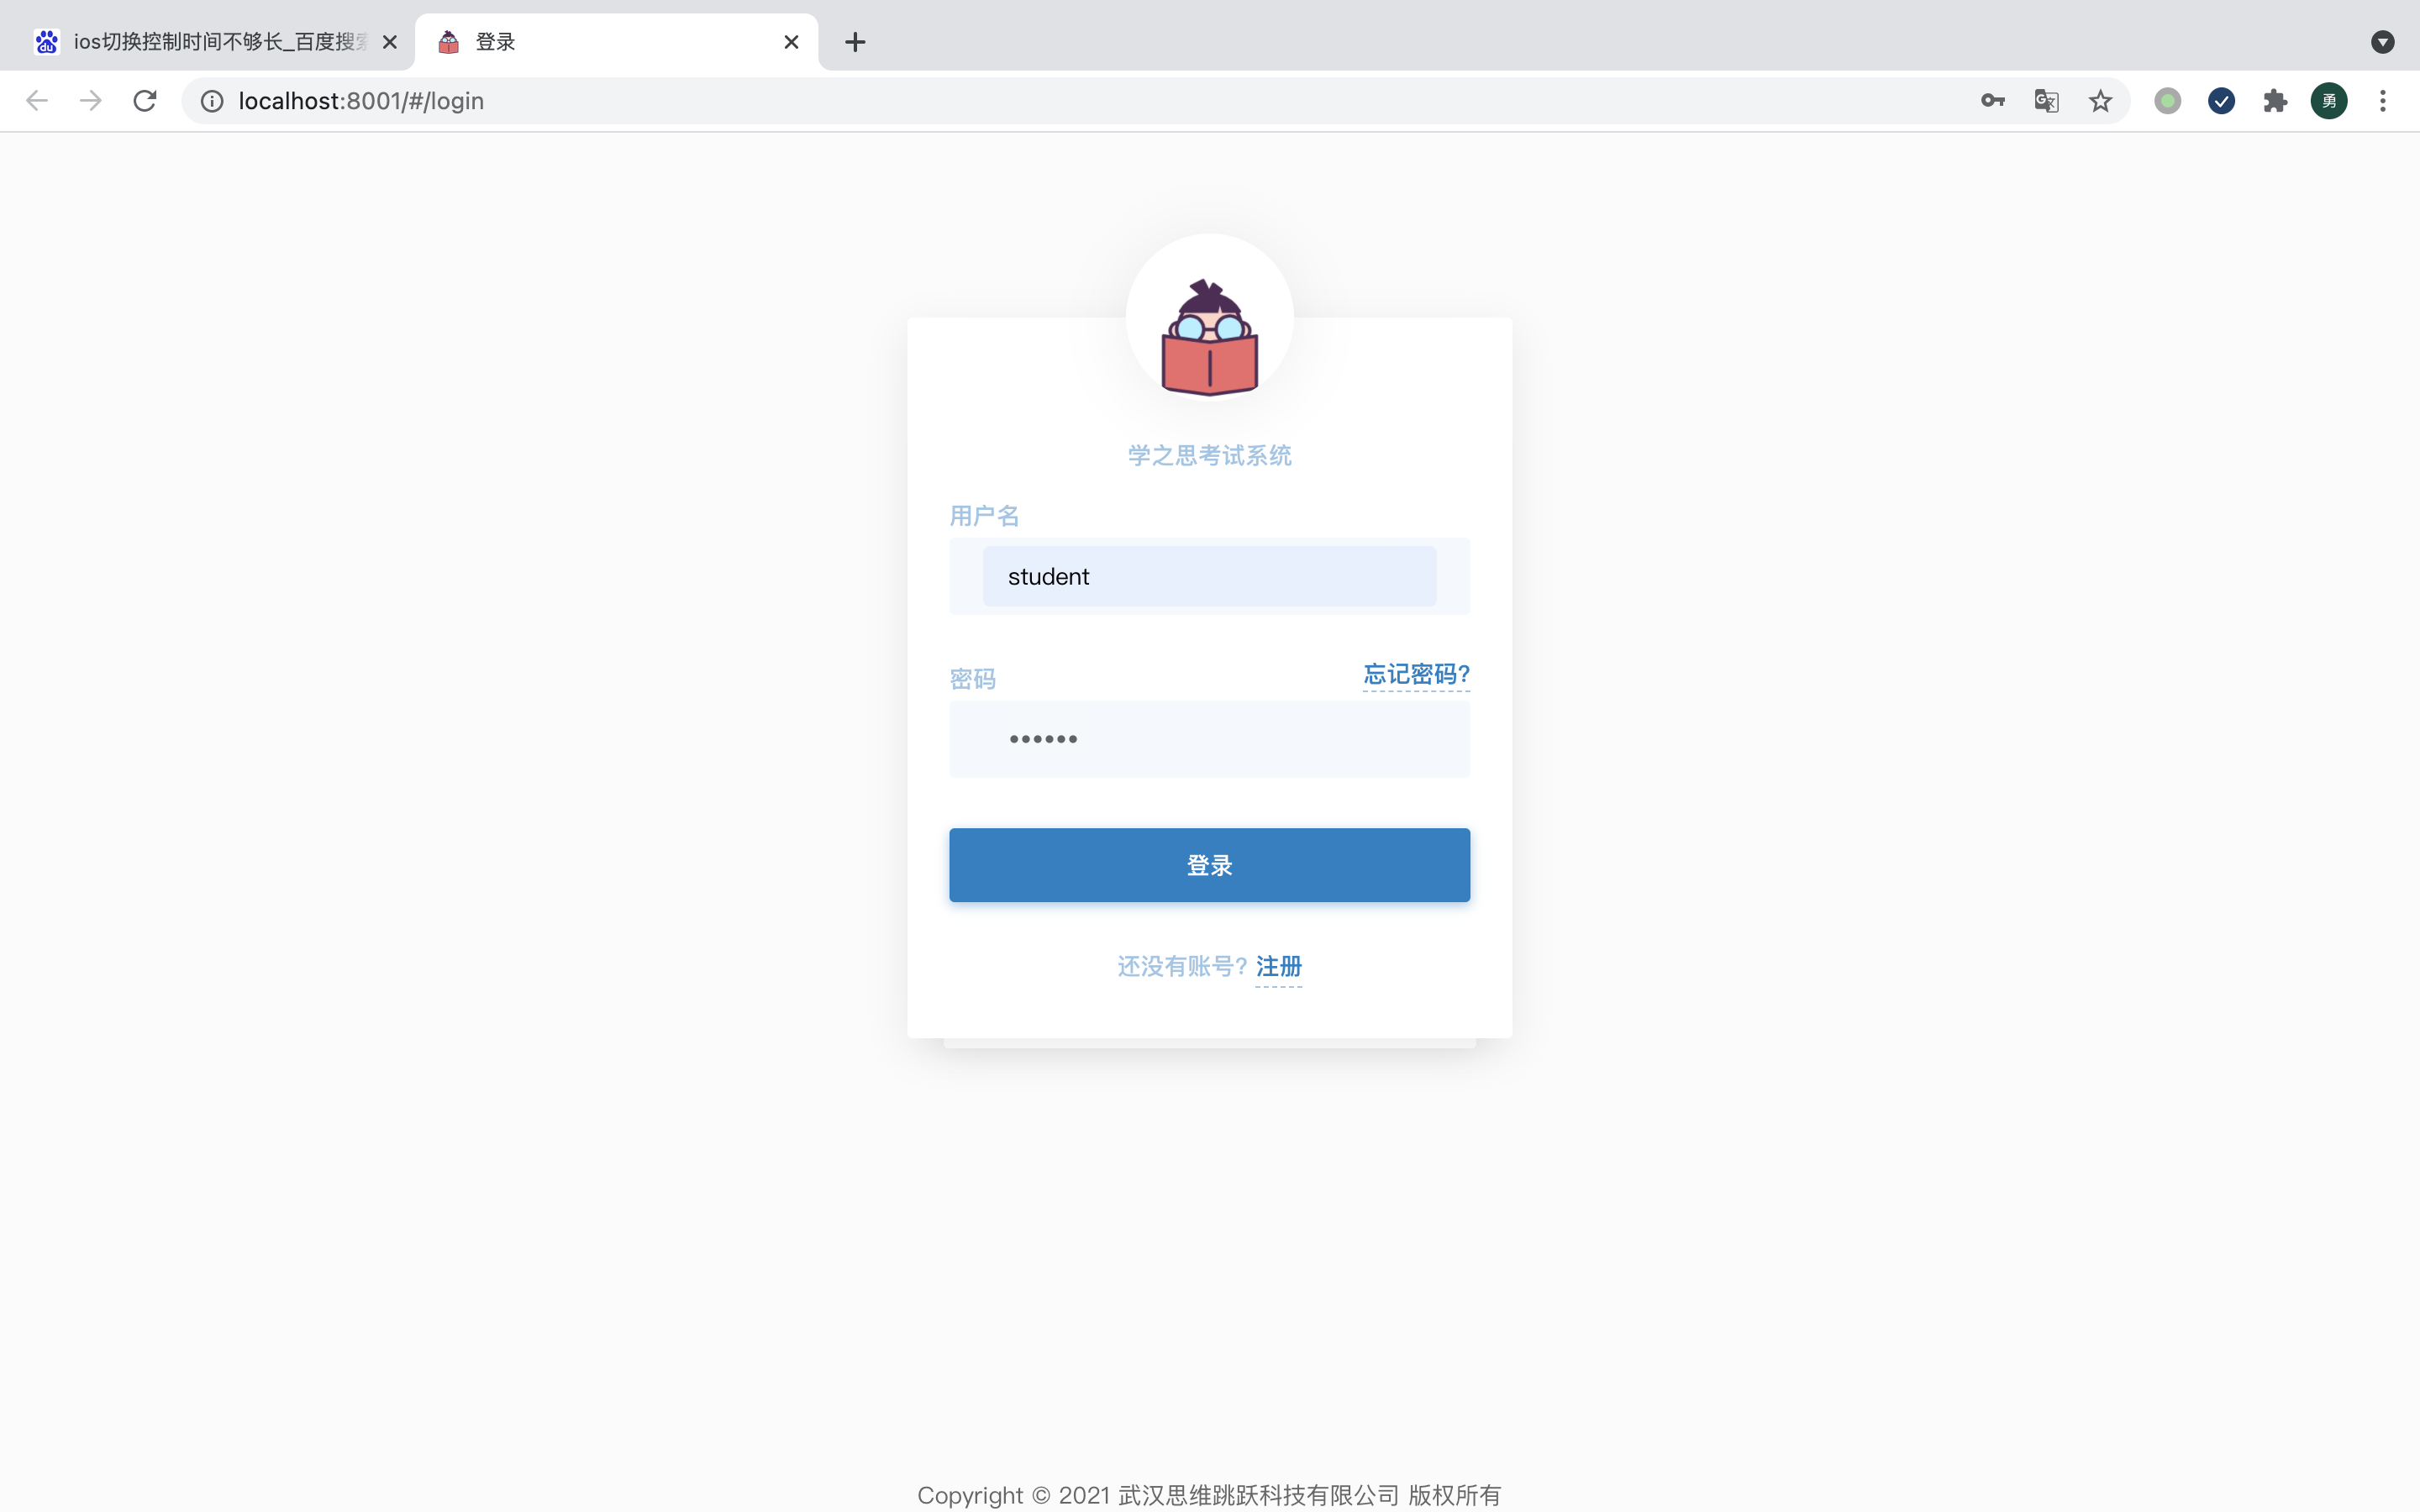
\includegraphics[width=1.0\textwidth,keepaspectratio]{data/chapter-5/student/denglu.png}
			\caption{学生登录}
			\label{figure:sdenglu}
		\end{figure}
\end{enumerate}

\subsection{学生主页}
\begin{enumerate}
	\item[] \textbf{功能描述:}学生系统的主页界面,展示一些主要信息,例如该学生可以进行的考试。
	\item[] \textbf{功能页面:}如图\ref{figure:szhuye}所示 \\
		\begin{figure}[H]
			\centering
			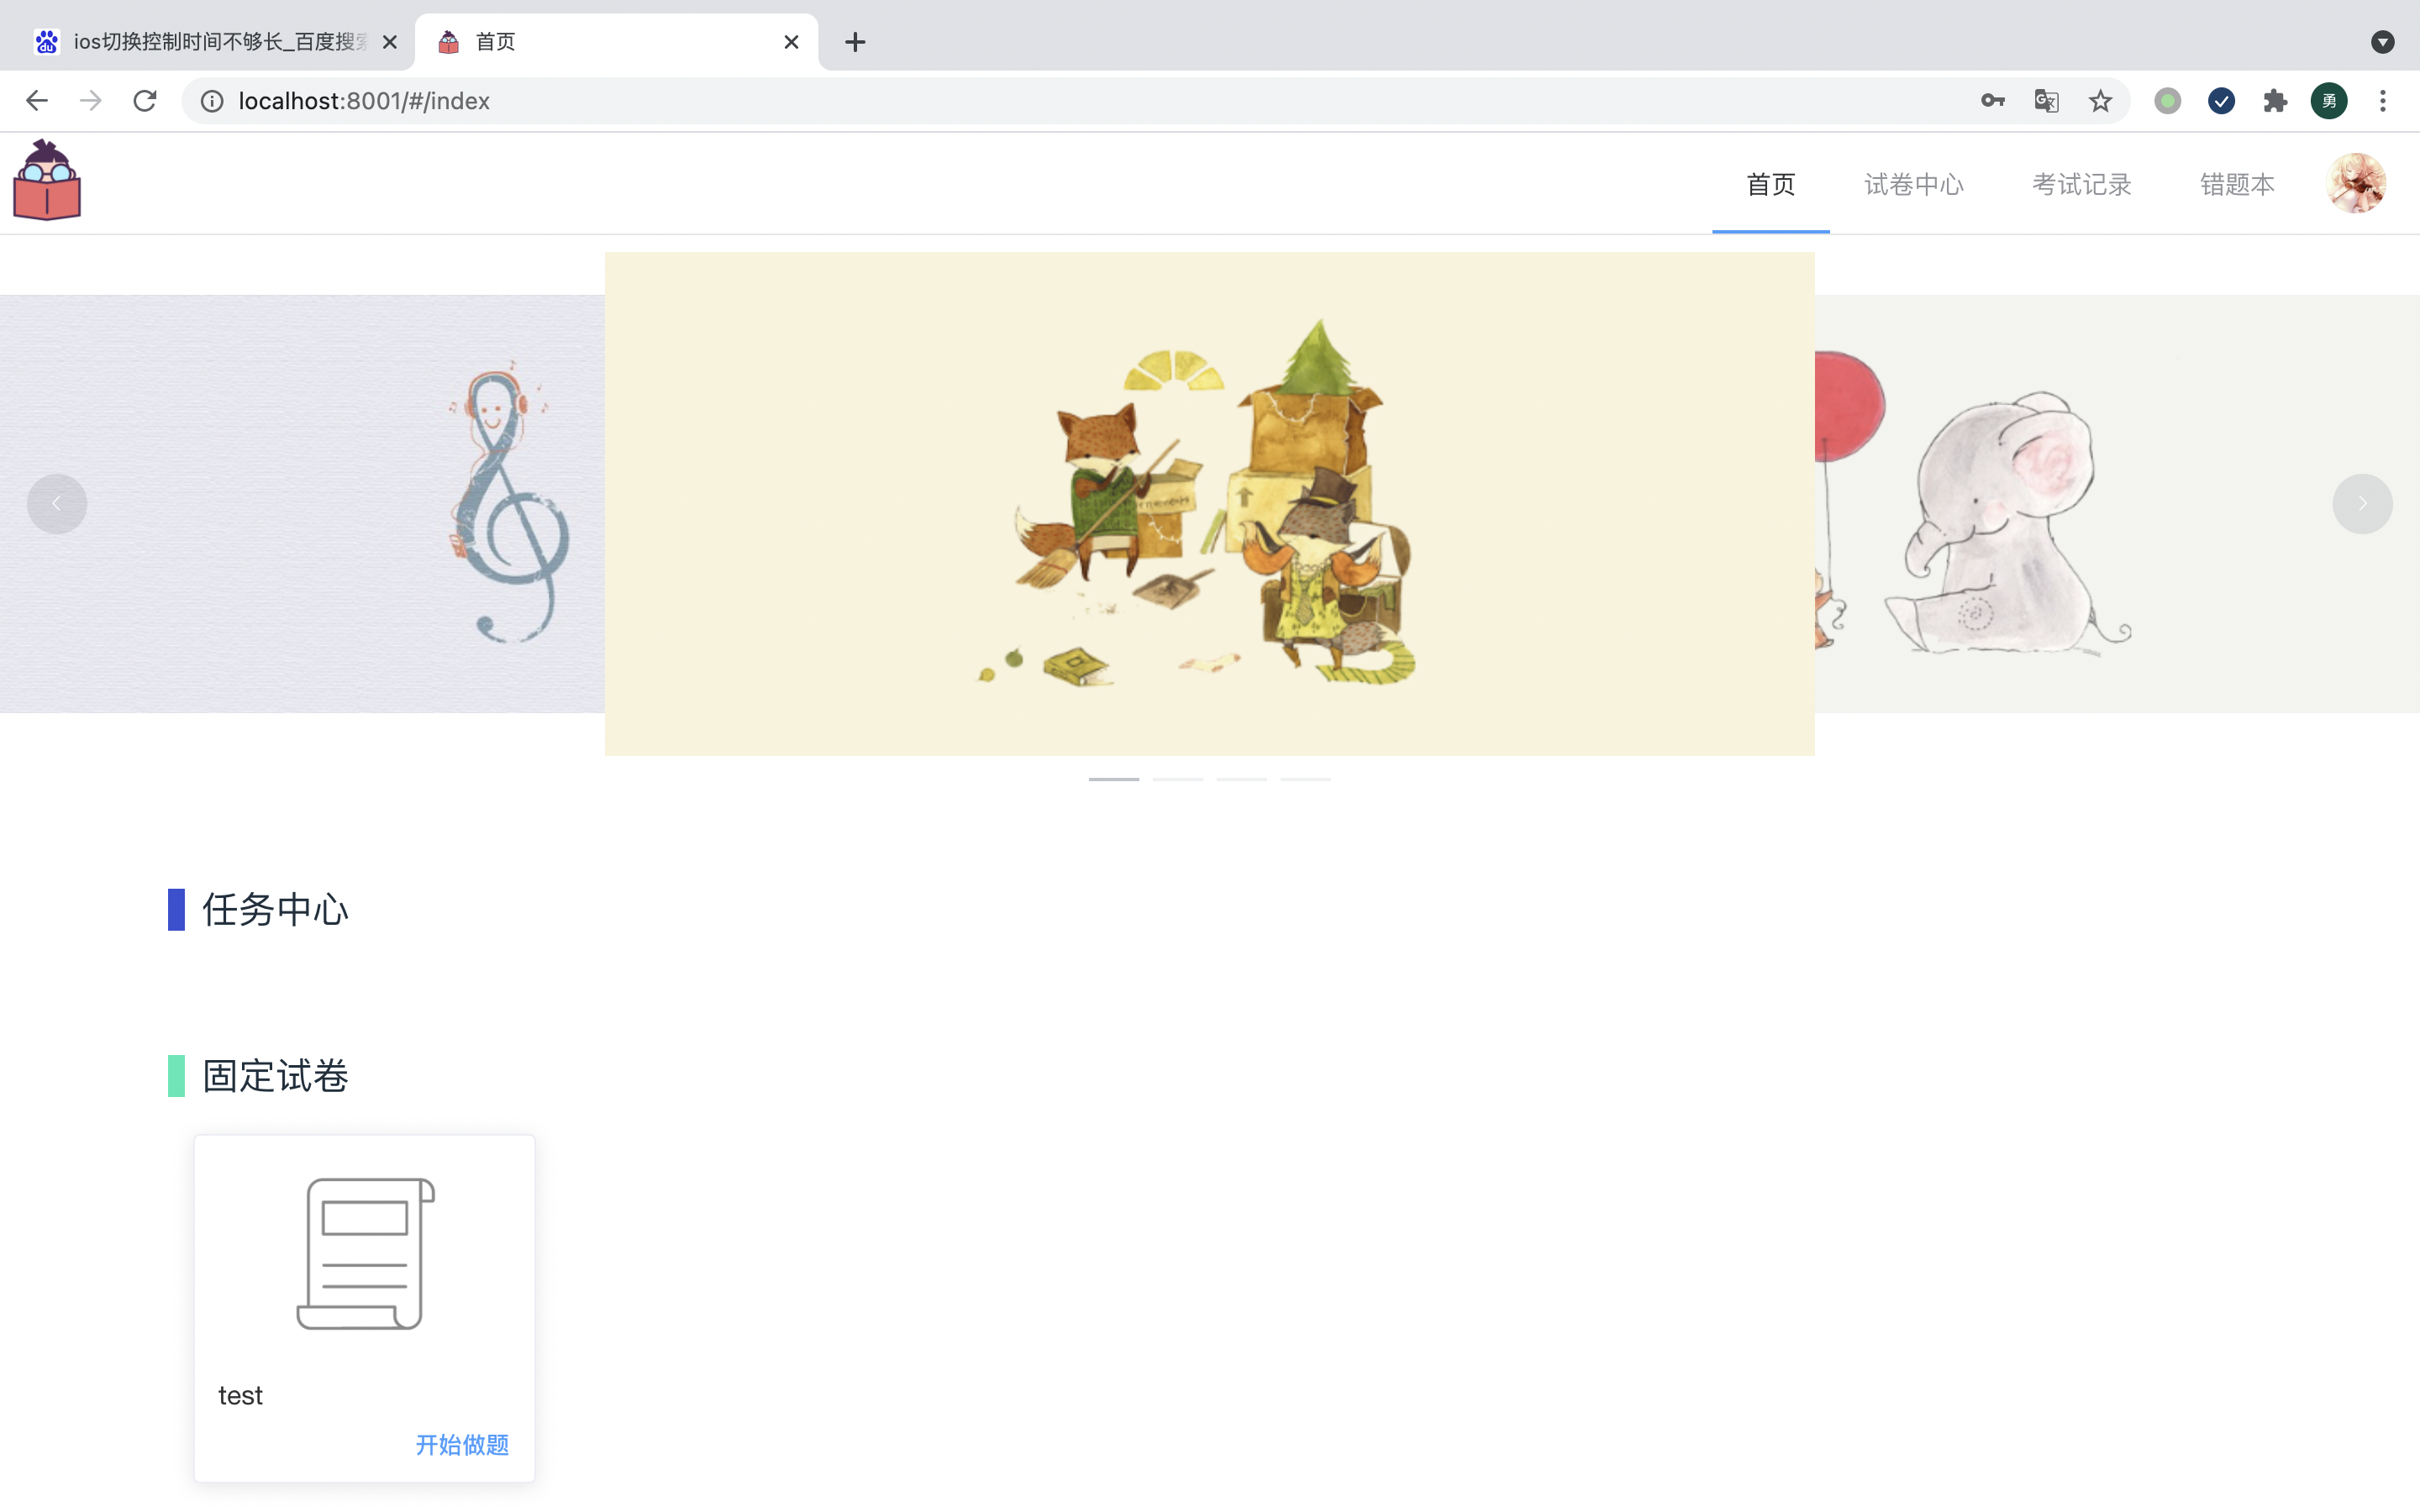
\includegraphics[width=1.0\textwidth,keepaspectratio]{data/chapter-5/student/zhuye.png}
			\caption{学生主页}
			\label{figure:szhuye}
		\end{figure}
\end{enumerate}

\subsection{学生试卷中心}
\begin{enumerate}
	\item[] \textbf{功能描述:}试卷中心功能界面,学生可以通过试卷中心找到所有公开的固定试卷和时段试卷。
	\item[] \textbf{功能页面:}如图\ref{figure:szhongxin}所示 \\
		\begin{figure}[H]
			\centering
			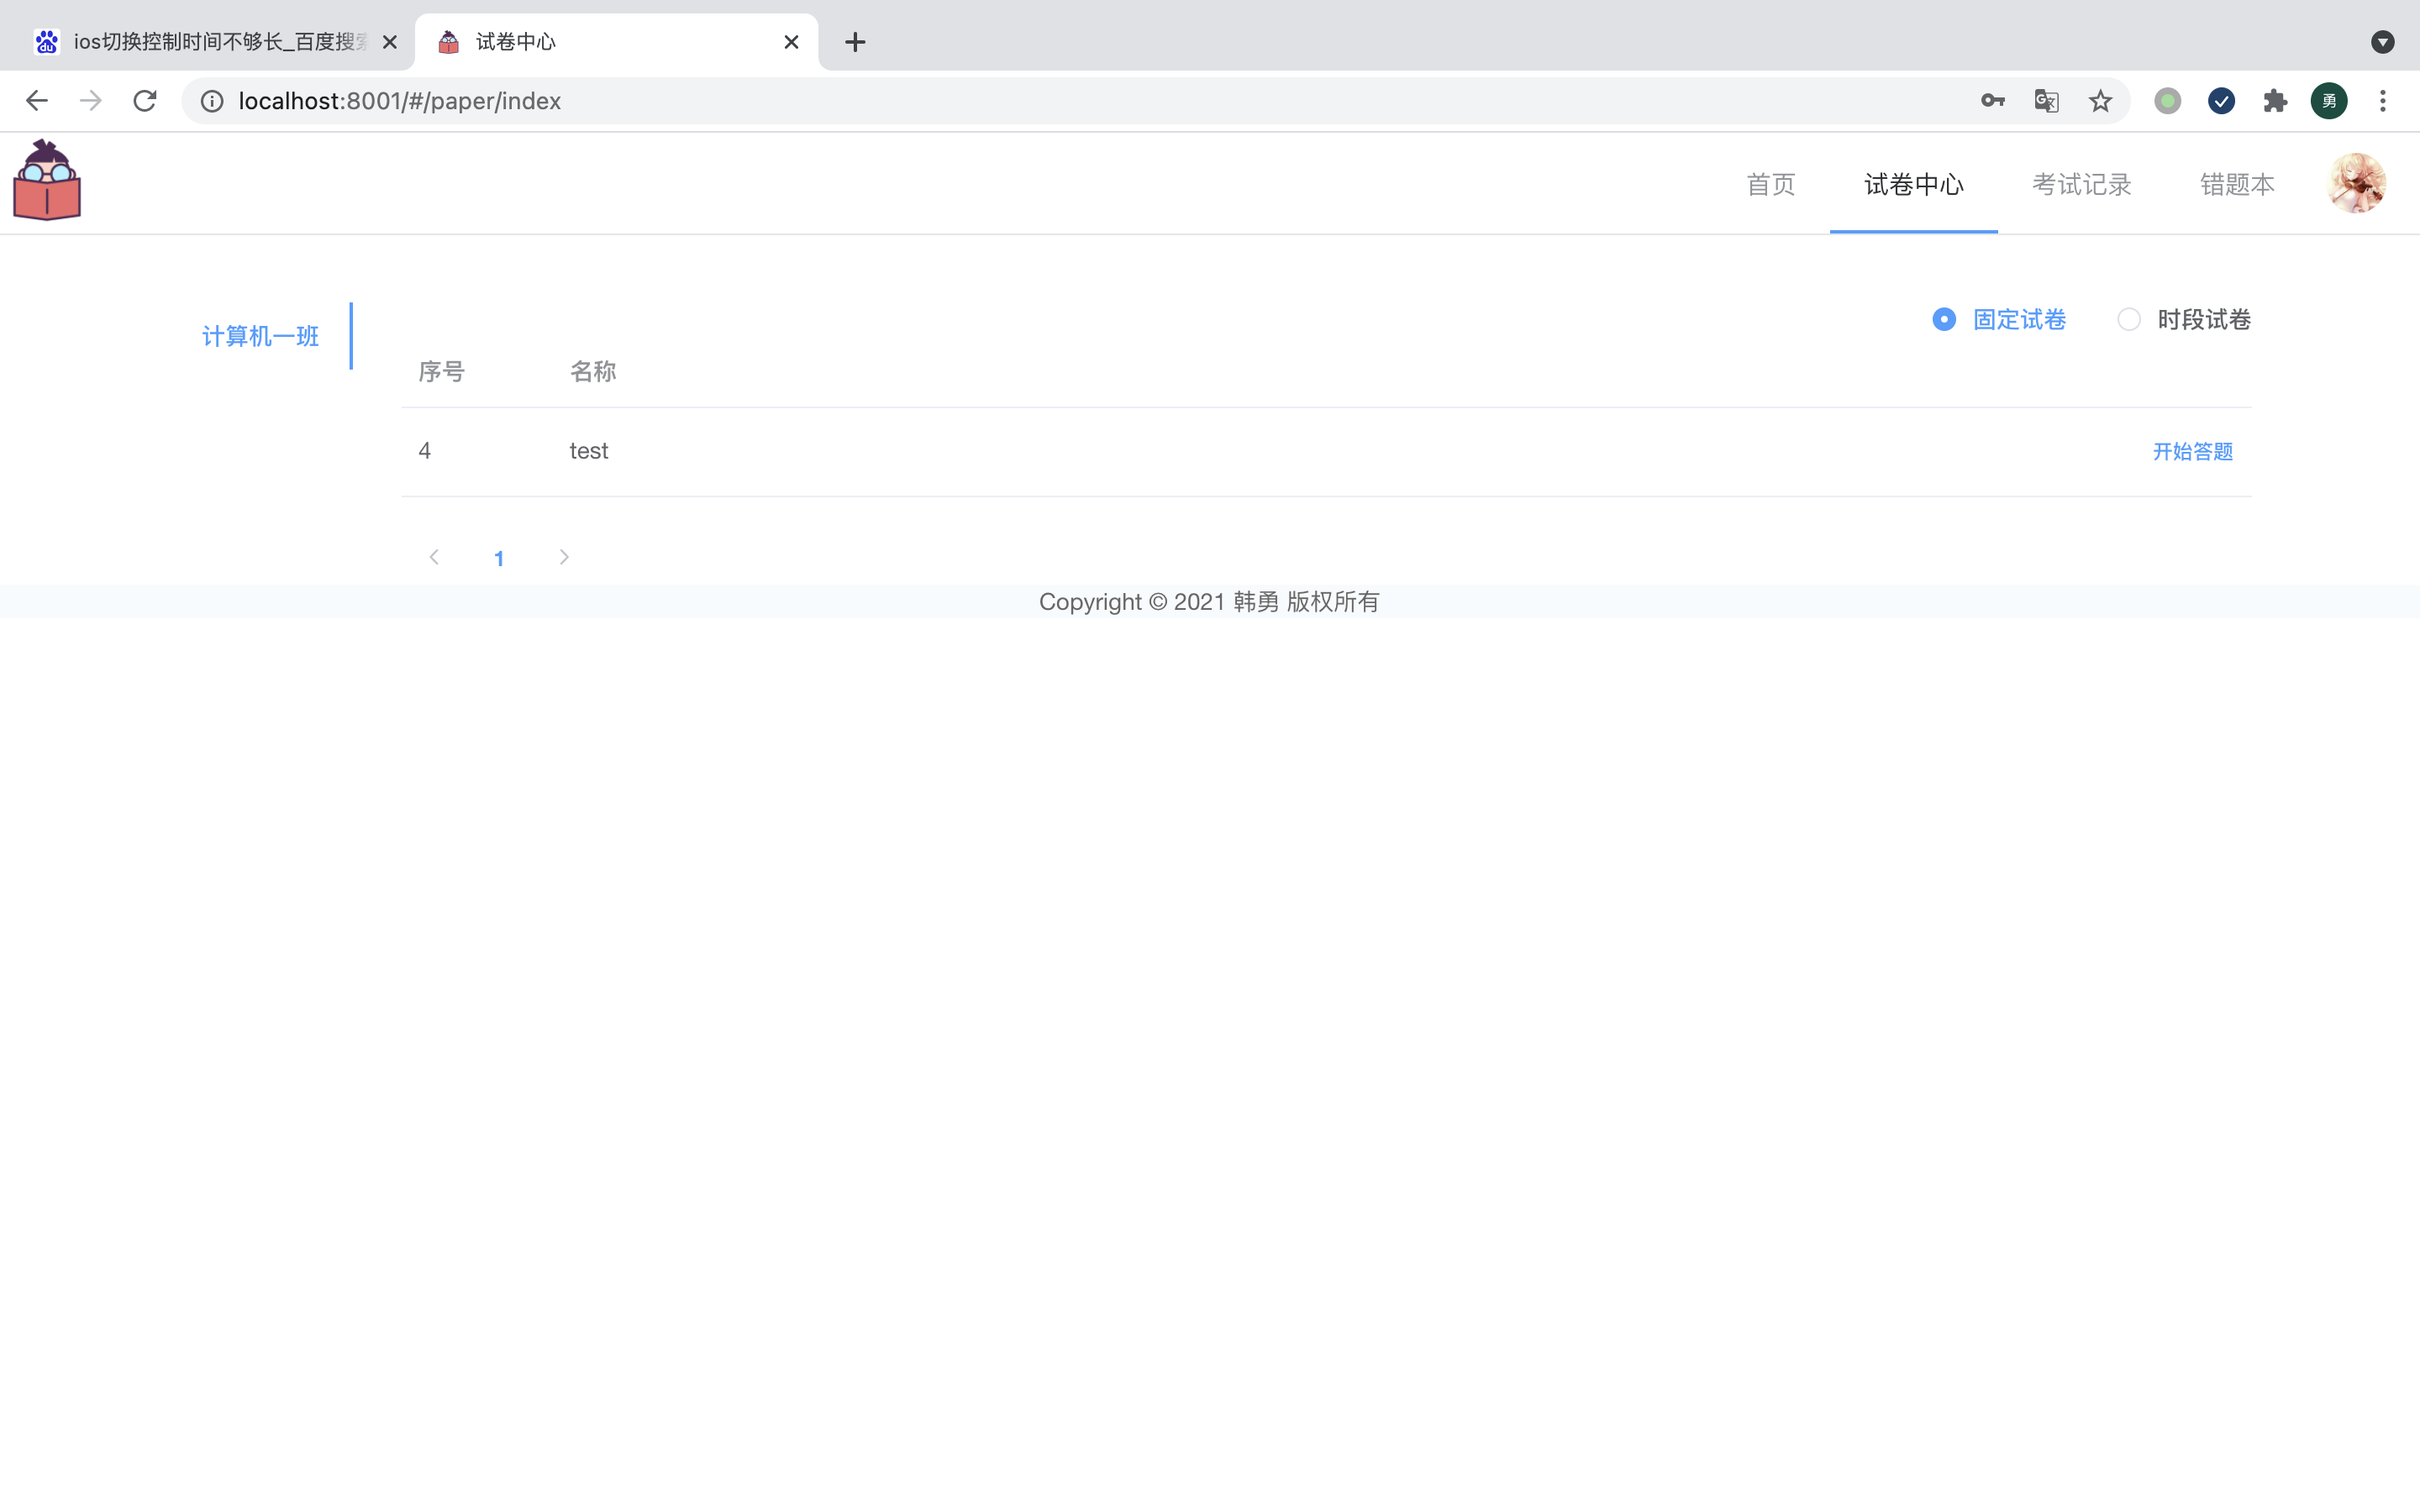
\includegraphics[width=1.0\textwidth,keepaspectratio]{data/chapter-5/student/shijuanzhongxin.png}
			\caption{学生试卷中心}
			\label{figure:szhongxin}
		\end{figure}
\end{enumerate}

\subsection{学生考试记录}
\begin{enumerate}
	\item[] \textbf{功能描述:}考试记录功能界面,学生可以通过该功能查看自己的考试记录和得分。
	\item[] \textbf{功能页面:}如图\ref{figure:sjilu}所示 \\
		\begin{figure}[H]
			\centering
			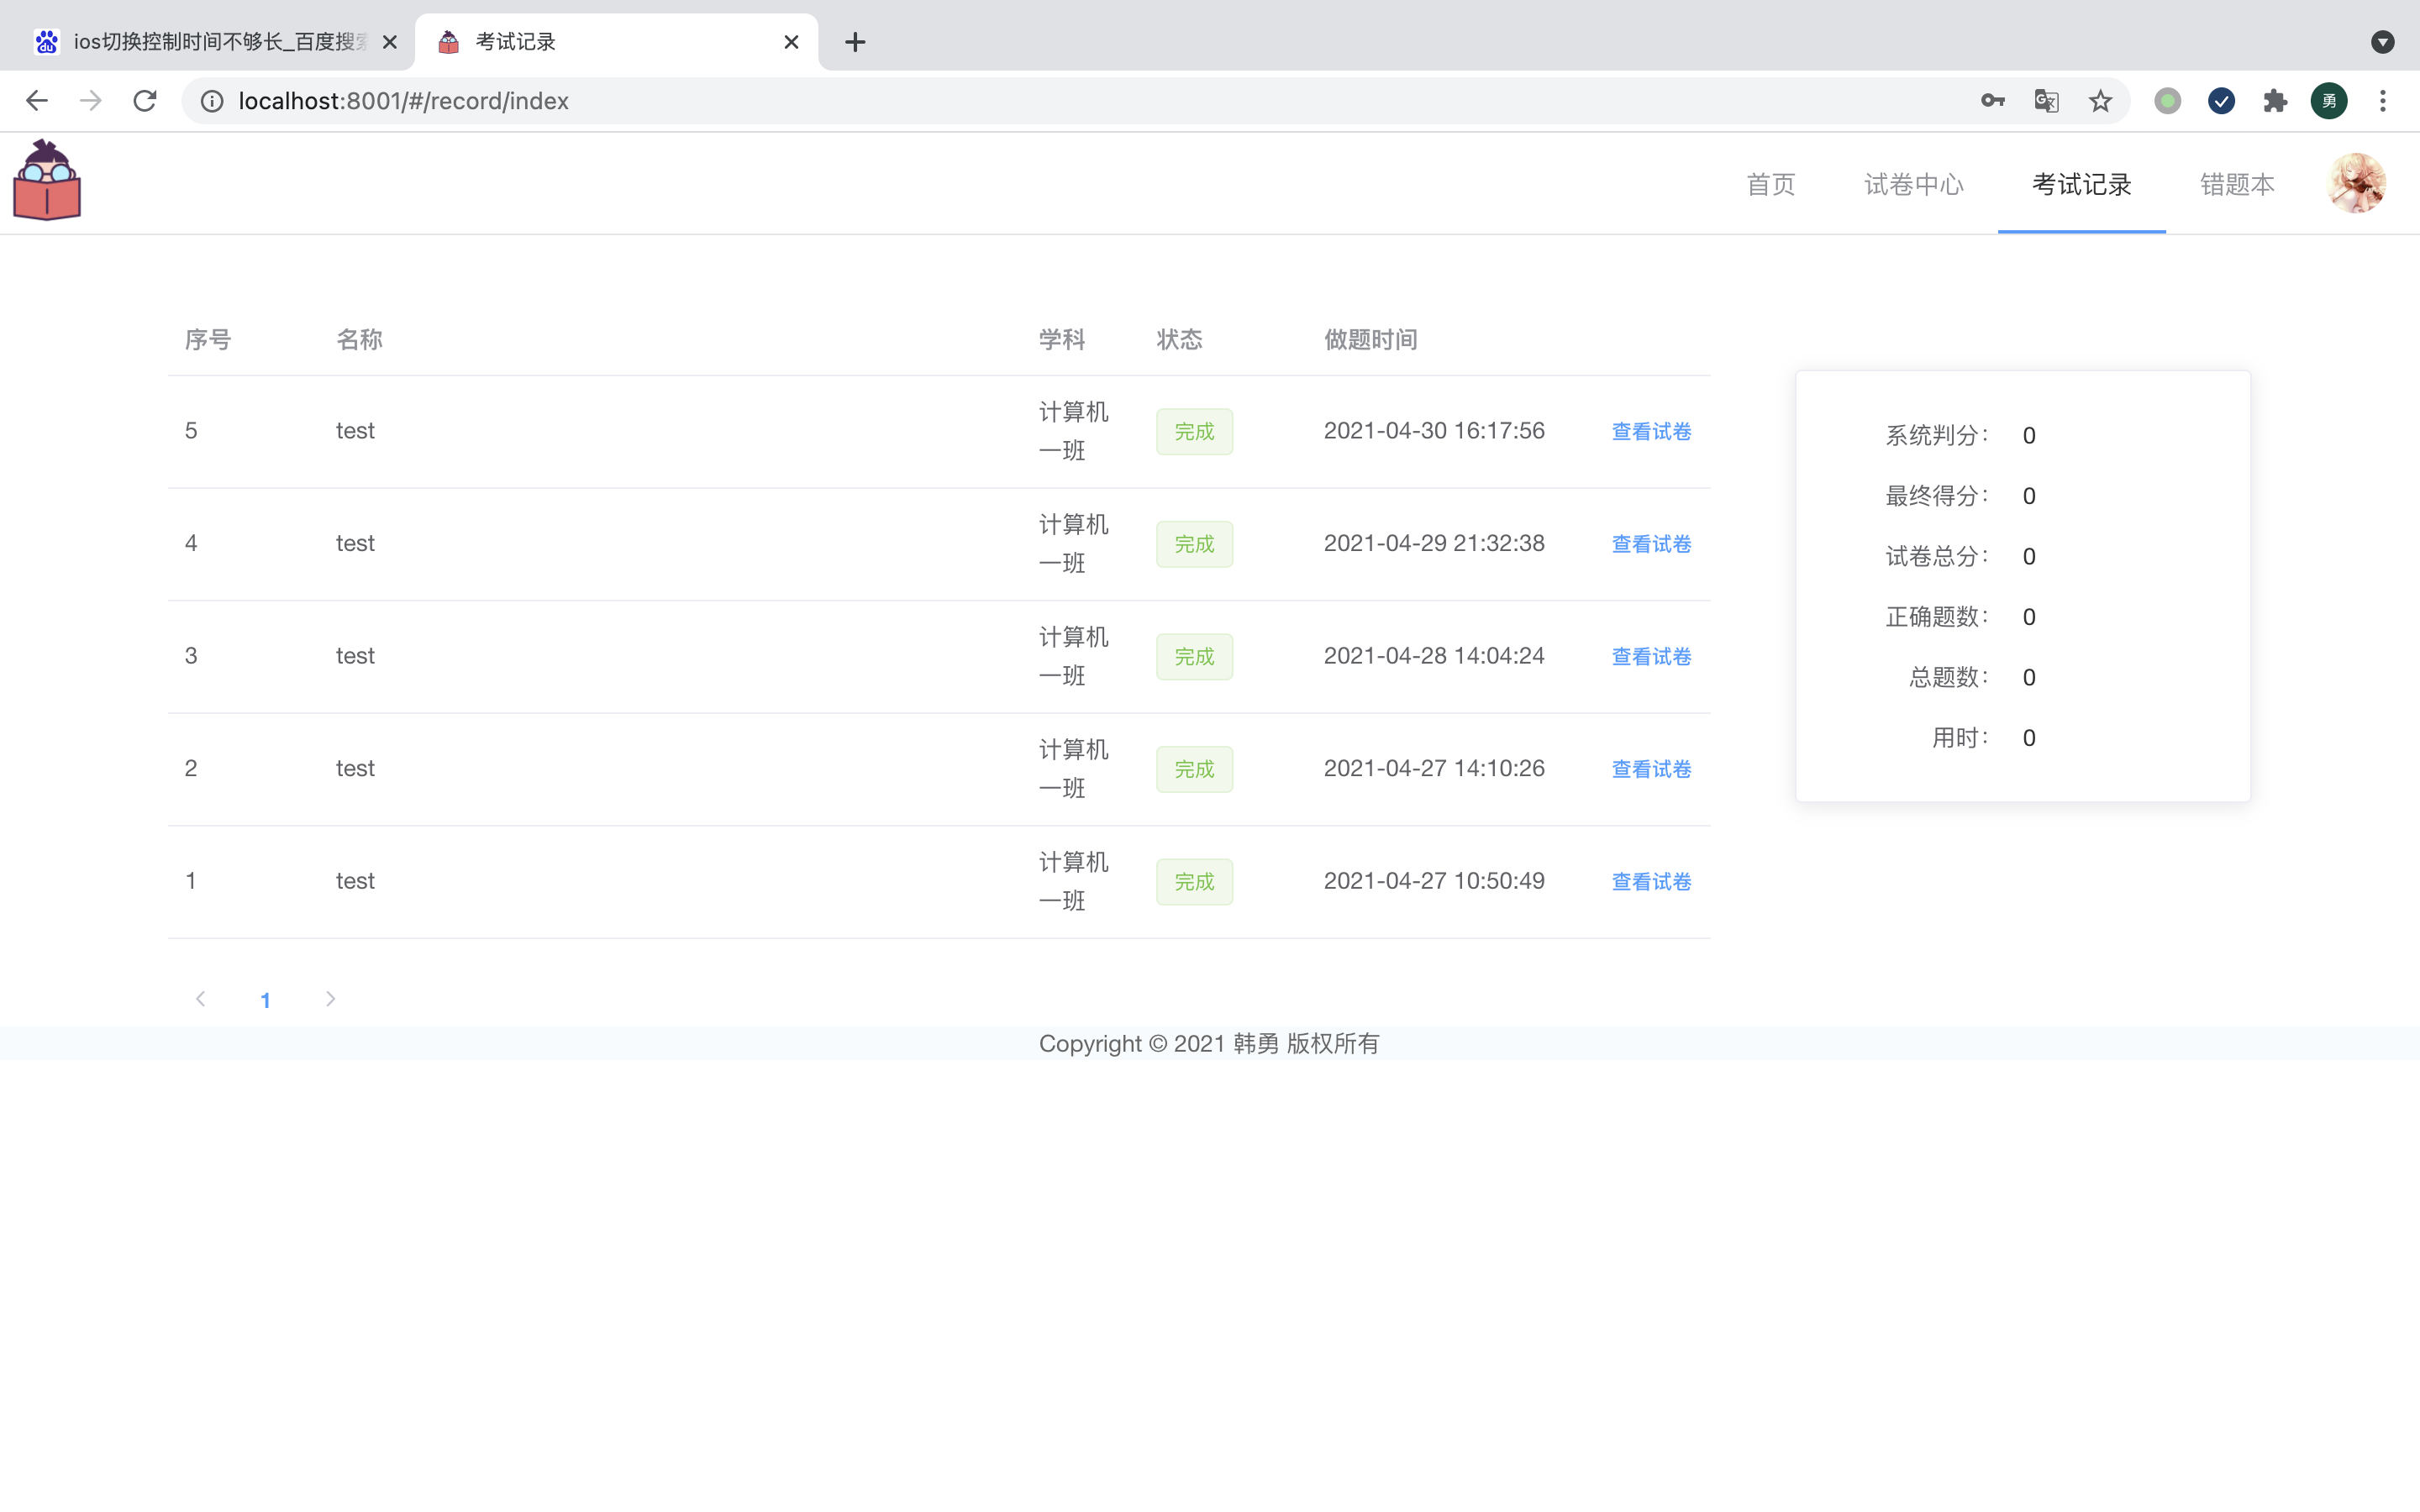
\includegraphics[width=1.0\textwidth,keepaspectratio]{data/chapter-5/student/kaoshijilu.png}
			\caption{学生考试记录}
			\label{figure:sjilu}
		\end{figure}
\end{enumerate}

\subsection{学生错题本}
\begin{enumerate}
	\item[] \textbf{功能描述:}错题本功能界面,学生可以通过该功能查看自己的历史错题,其中包括错误原因、正确答案和题目解析。
	\item[] \textbf{功能页面:}如图\ref{figure:scuotiben}所示 \\
		\begin{figure}[H]
			\centering
			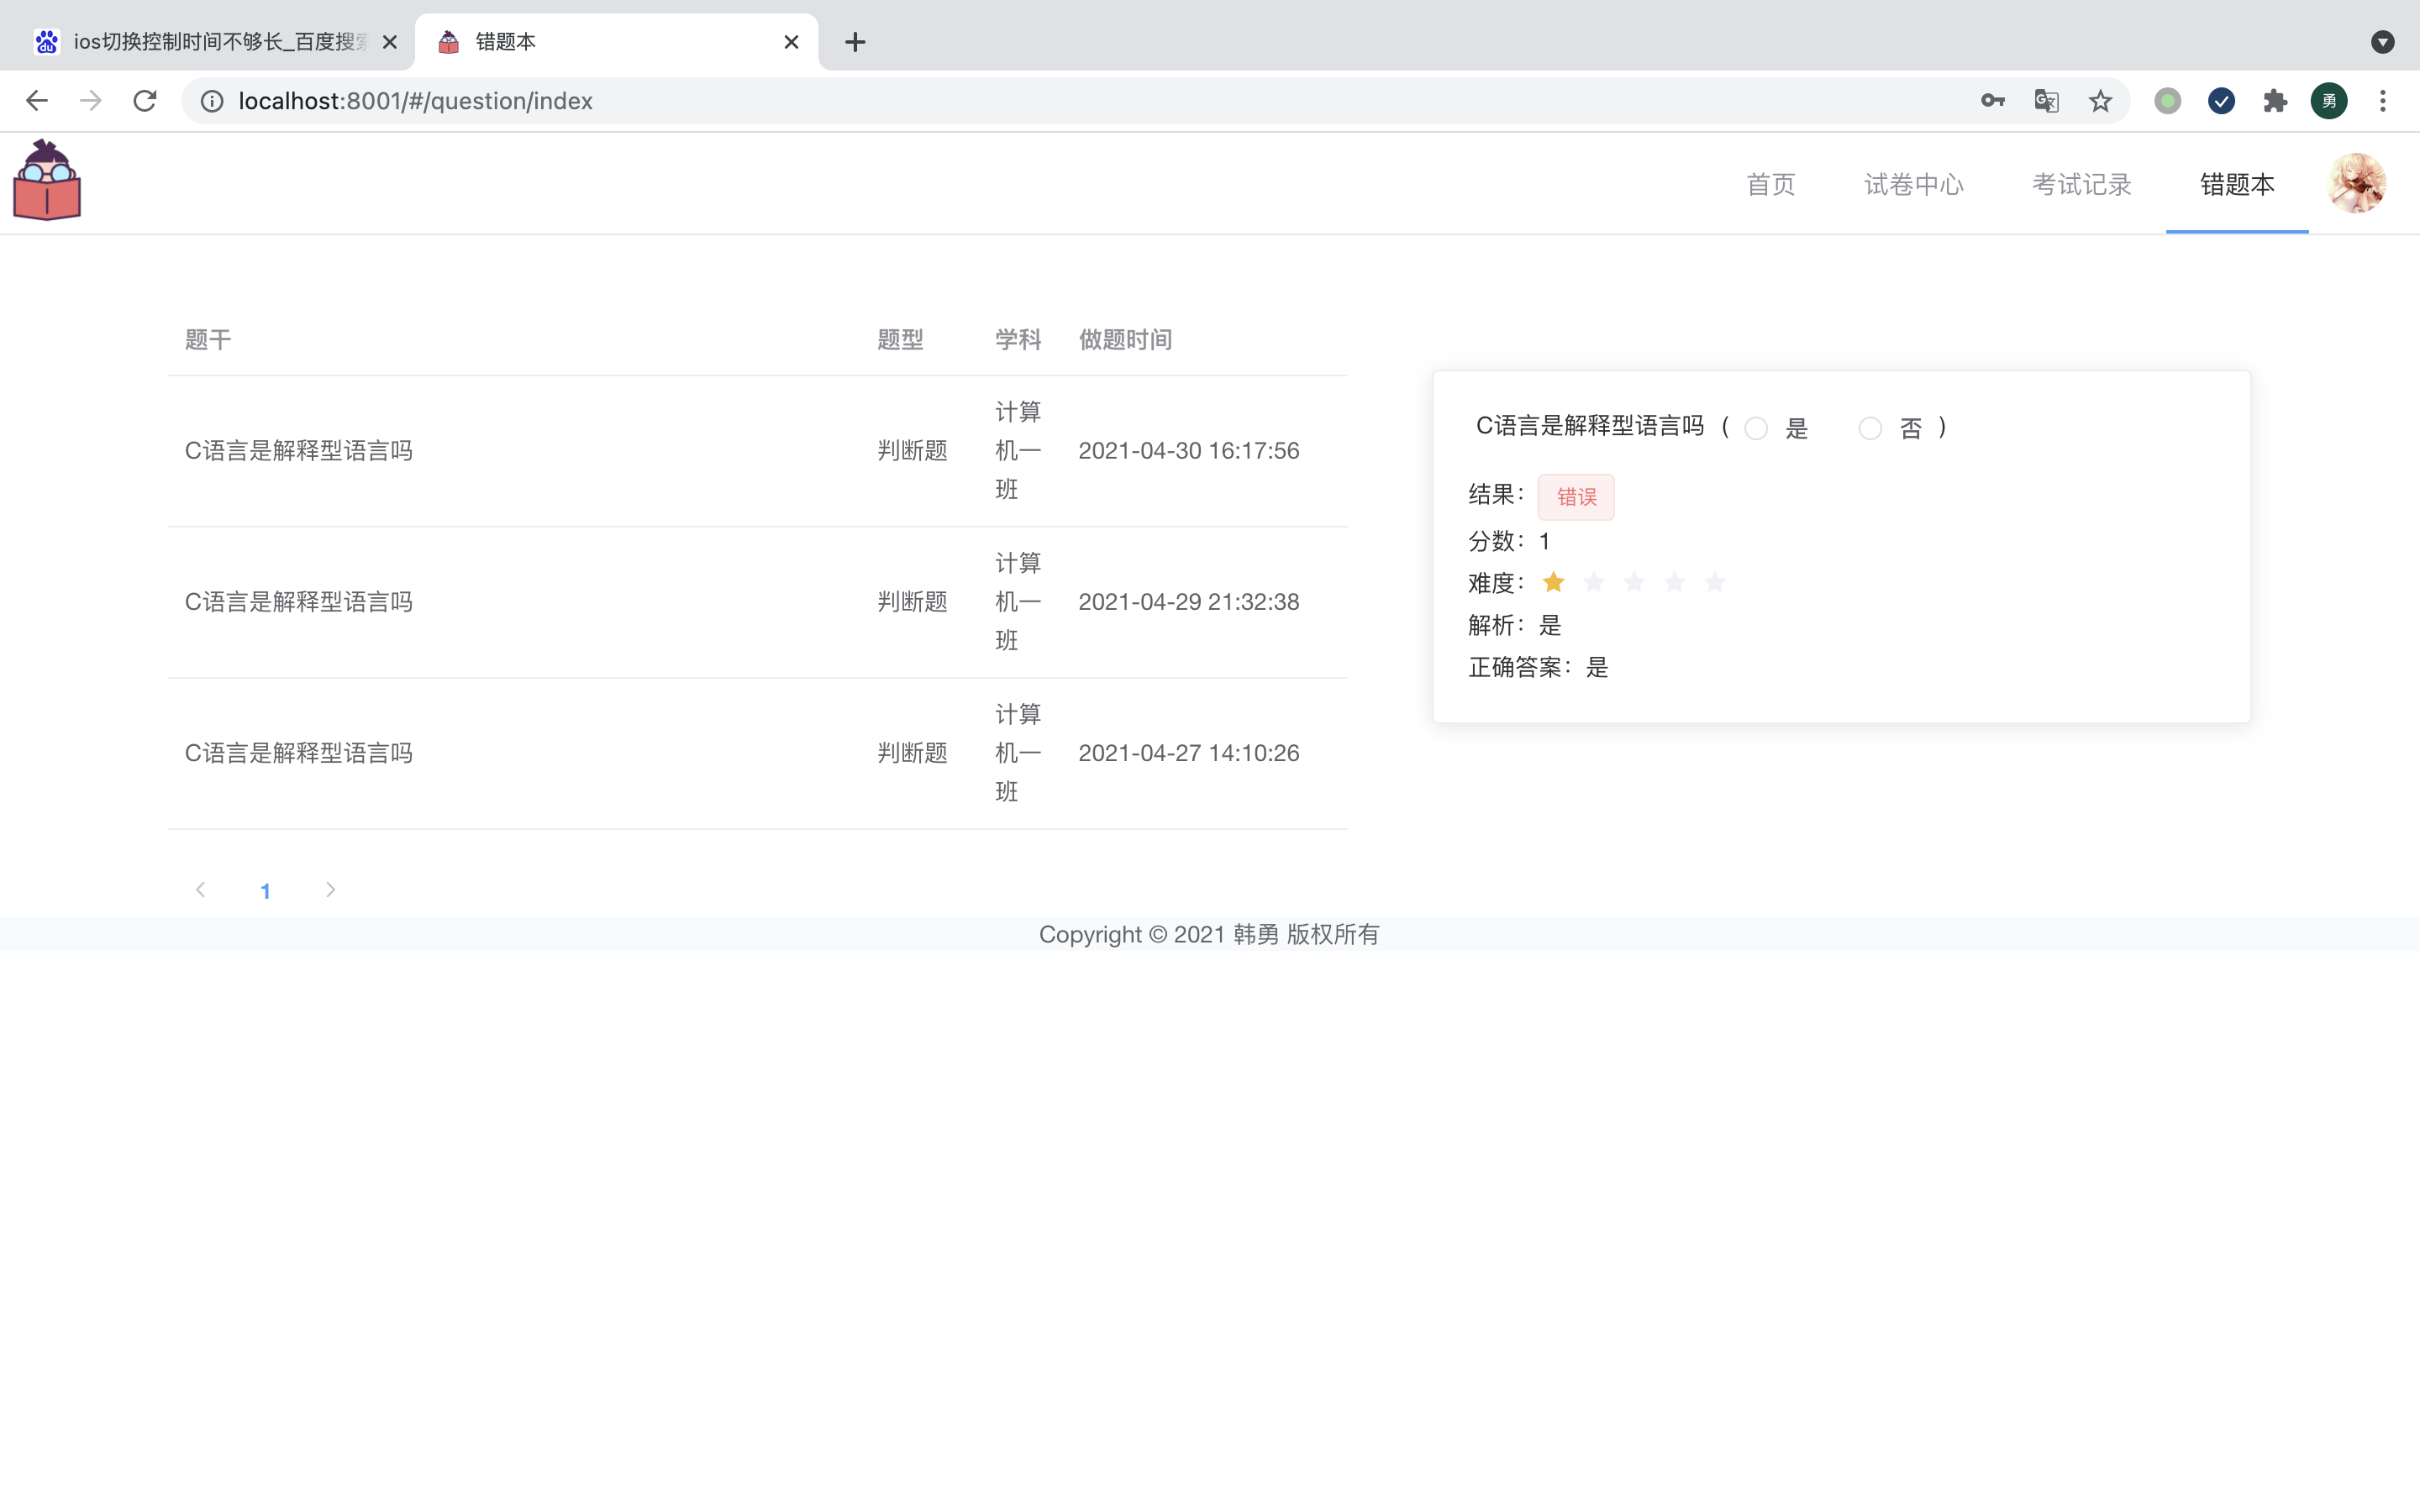
\includegraphics[width=1.0\textwidth,keepaspectratio]{data/chapter-5/student/cuotiben.png}
			\caption{学生错题本}
			\label{figure:scuotiben}
		\end{figure}
\end{enumerate}

\subsection{学生用户信息}
\begin{enumerate}
	\item[] \textbf{功能描述:}用户信息功能界面,学生可以通过该功能查看自己的个人信息并可以修改相关信息。
	\item[] \textbf{功能页面:}如图\ref{figure:sxinxi}所示 \\
		\begin{figure}[H]
			\centering
			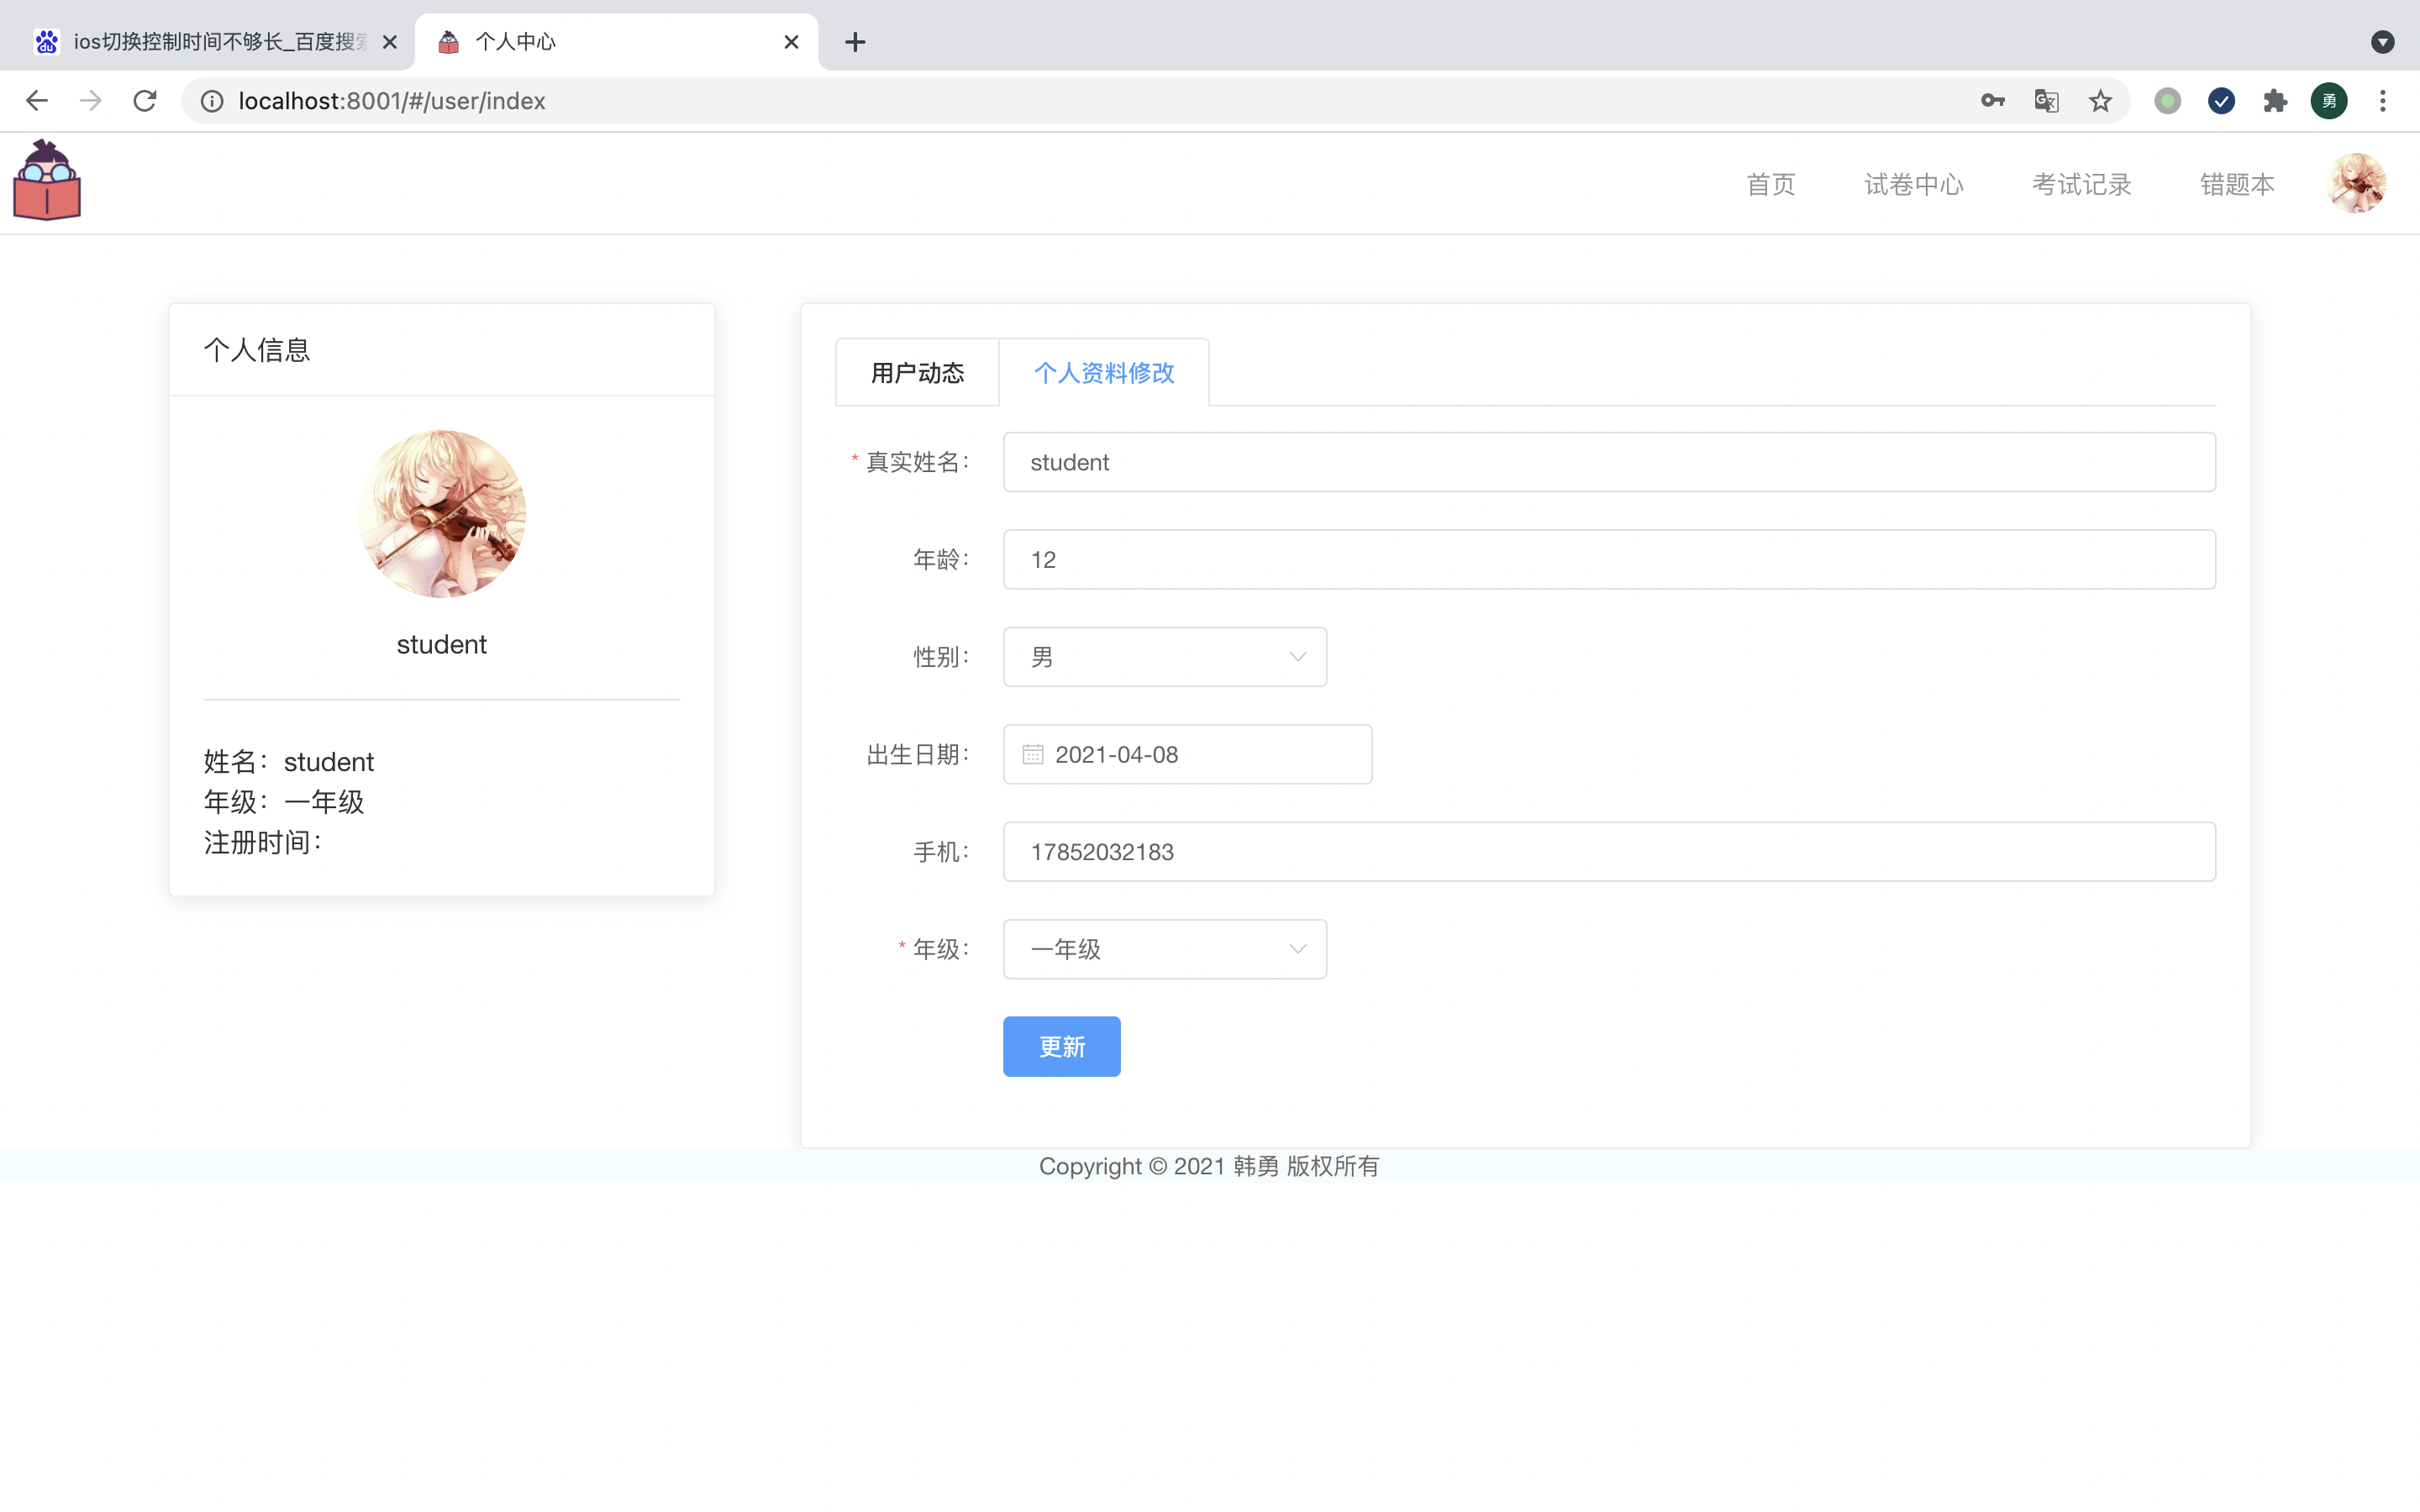
\includegraphics[width=1.0\textwidth,keepaspectratio]{data/chapter-5/student/yonghuxinxi.png}
			\caption{学生用户信息}
			\label{figure:sxinxi}
		\end{figure}
\end{enumerate}

\subsection{学生考试}
\begin{enumerate}
	\item[] \textbf{功能描述:}考试功能界面,学生开始考试或练习后会进入该界面,进入该页面后将自动开始录像并随机拍照对考试进行监控,考试时间结束后,考试将自动结束
	并提交,学生也可以在考试时间结束之前自行提交。
	\item[] \textbf{功能页面:}如图\ref{figure:skaoshi}所示 \\
		\begin{figure}[H]
			\centering
			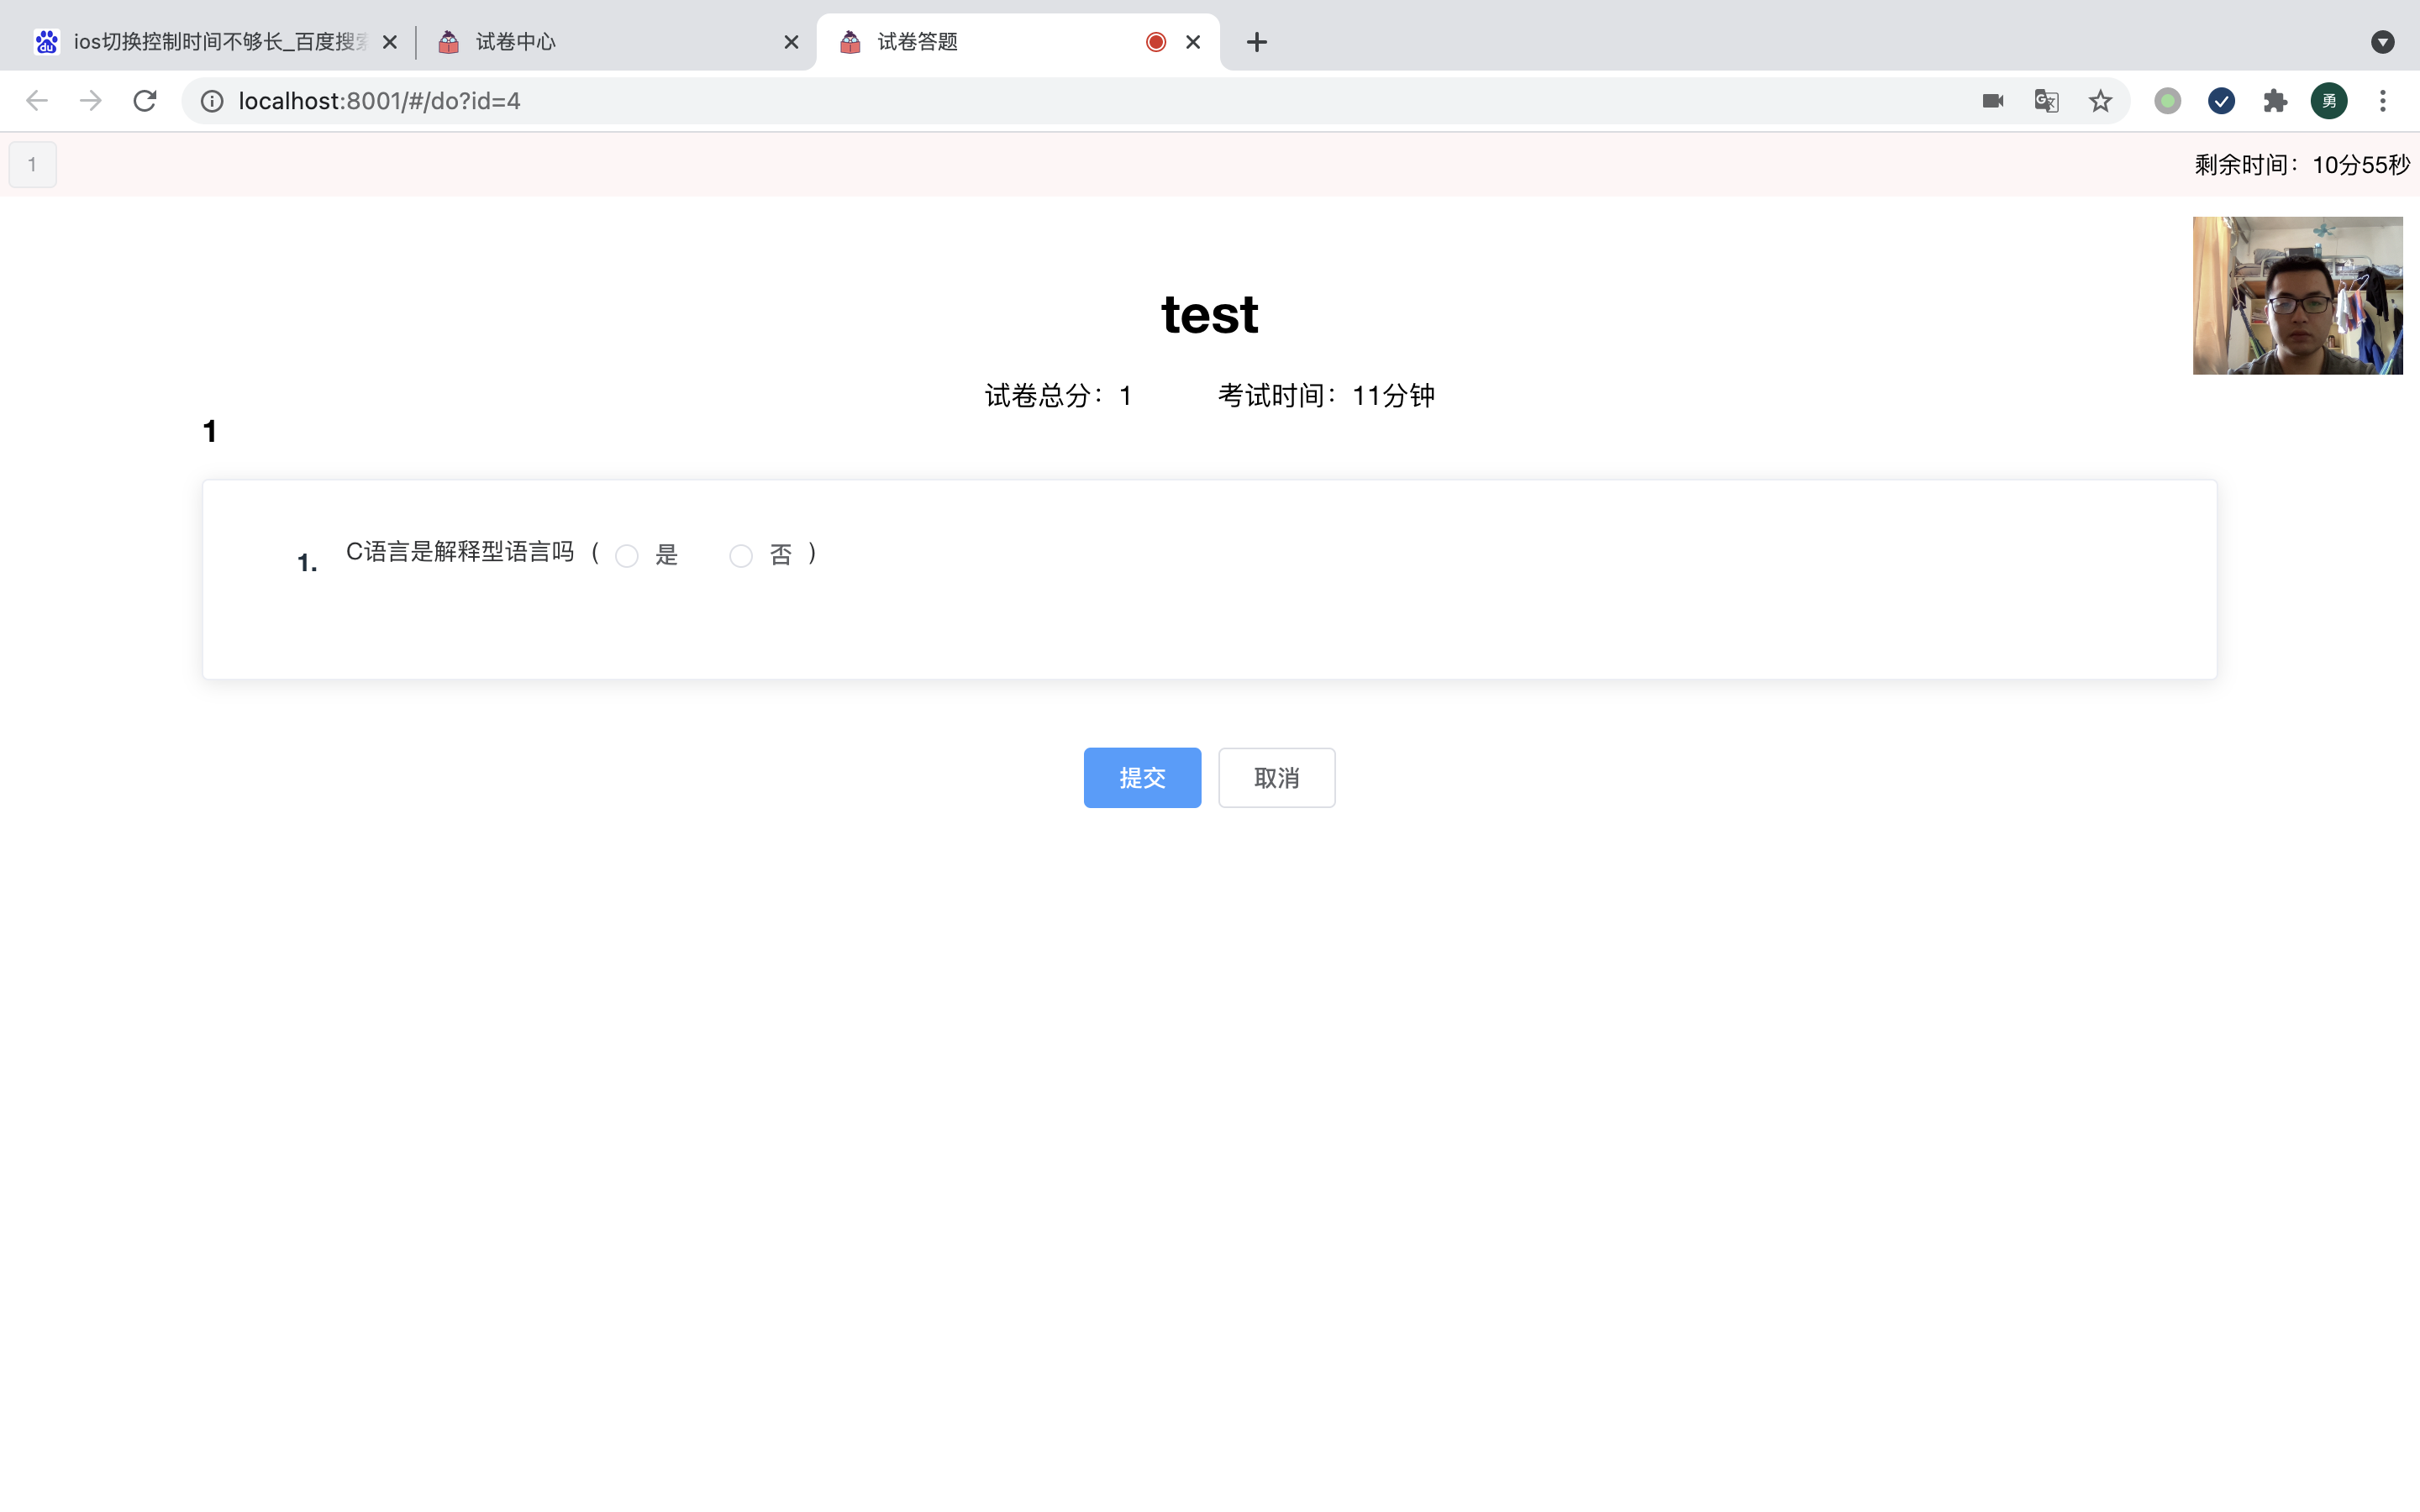
\includegraphics[width=1.0\textwidth,keepaspectratio]{data/chapter-5/student/kaoshi.png}
			\caption{学生考试}
			\label{figure:skaoshi}
		\end{figure}
\end{enumerate}
    \cleardoublepage

    \renewcommand{\thechapter}{}
    \bibliographystyle{data/gbt7714-2005}
\bibliography{data/bibliography}
\addcontentsline{toc}{chapter}{\bibname}

    \cleardoublepage

    \include{data/acknowledgment}
    \cleardoublepage
  }

\end{document}
